\documentclass[../structure.tex]{subfiles}
\begin{document}
\chapter{Results}
\hspace{2em}After implementing non-rigid ICP, we test the tools we have developed to assess the algorithm. We use data collected from \textbf{\textit{Human Connectome Projects}} \cite{CCF}. The number of samples used for testing is four with eleven pathways (bundles) in each side of the brain. We present two experiments to show how the method works from the same patient. The first experiment is left and right side of the same pathway and the second one is for one pathway, which deformed and re-registered again with the original shape.

\begin{center}
\begin{table}[h!]
	\begin{tabular}{| c | c  c  c | c  c  c |}
	%\begin{tabular}{*7c}
	\toprule
	&\multicolumn{3}{c}{Tracts}&\multicolumn{3}{c}{Points}\\
Pathways&Average&Max&Min&Average&Max&Min\\
\midrule
%\hline
ATR&266.75&603&106&26443.875&69283&9623\\
rostrum&1853.375&2020&1633&162936.625&188143&137536\\
Cing&1103.375&1369&872&167488.25&244088&100762\\
CST&1649.25&2044&1476&235265.375&308769&170535\\
Fornix&399&497&308&26618&37142&16703\\
genu&2134.5&2333&1967&166567.625&236384&144492\\
IFOF&862.875&985&774&128850.875&162086&90424\\
ILF&3751&4392&2950&566332.25&673060&367155\\
SLF&1333.125&1633&1044&174943.5&251994&105245\\
splenium&2209.625&2335&2063&206526.875&244341&182993\\
VTA&327.625&679&150&27784.125&54904&14982\\
\bottomrule
	\end{tabular}
\caption{The statistics of tracts (streamlines) and points in data}
\label{table:data}
\end{table}
\end{center}

\section{DIPY registration Method}
We compare our tools with a registration method discussed in \cite{Garyfallidis2015} and implemented in \textit{DIPY} package.

The method starts by reducing the number of points in each tract to a certain number of point, which is necessary for the method to have the same number of points in each tract.

DIPY method gets the initial orientation by placing both bundles (streamlines) in the origin point of the 3D Euclidean space. In this case, it considers only translation but not other transformations. To solve this problem and to be fare on the comparison, we use PCA tool that we develop to get the initial alignment before applying the DIPY method.

DIPY calculate the distance between template bundle and target bundle using a function called \textit{minimum average direct-flip distance (MDF)}. MDF is asymmetric
distance function, which can be applied only when all tracts have the same number of points, that is one reason why we reduce the number of point before applying DIPY registration, another reason is increasing the speed of distance calculation \cite{Garyfallidis2012}.

The method then uses optimizer to select the best combination of variables, which later converted to affine matrix, while reducing the overall distance between template bundle.

\begin{comment}
\section{Testing steps}
\begin{itemize}
\item Read bundles from \textit{ply} files
\item Apply PCA and visually inspect the alignment result
\item If the visual inspection was positive and PCA improved the alignment, we consider its result, otherwise we just flip the template bundle or consider the original orientation
\item Generate distances histogram between two bundles to select the distance threshold
\item Start the registration and iterate until there is no more improvement on the alignment
\end{itemize}
\end{comment}

\begin{figure}[H]
\centering
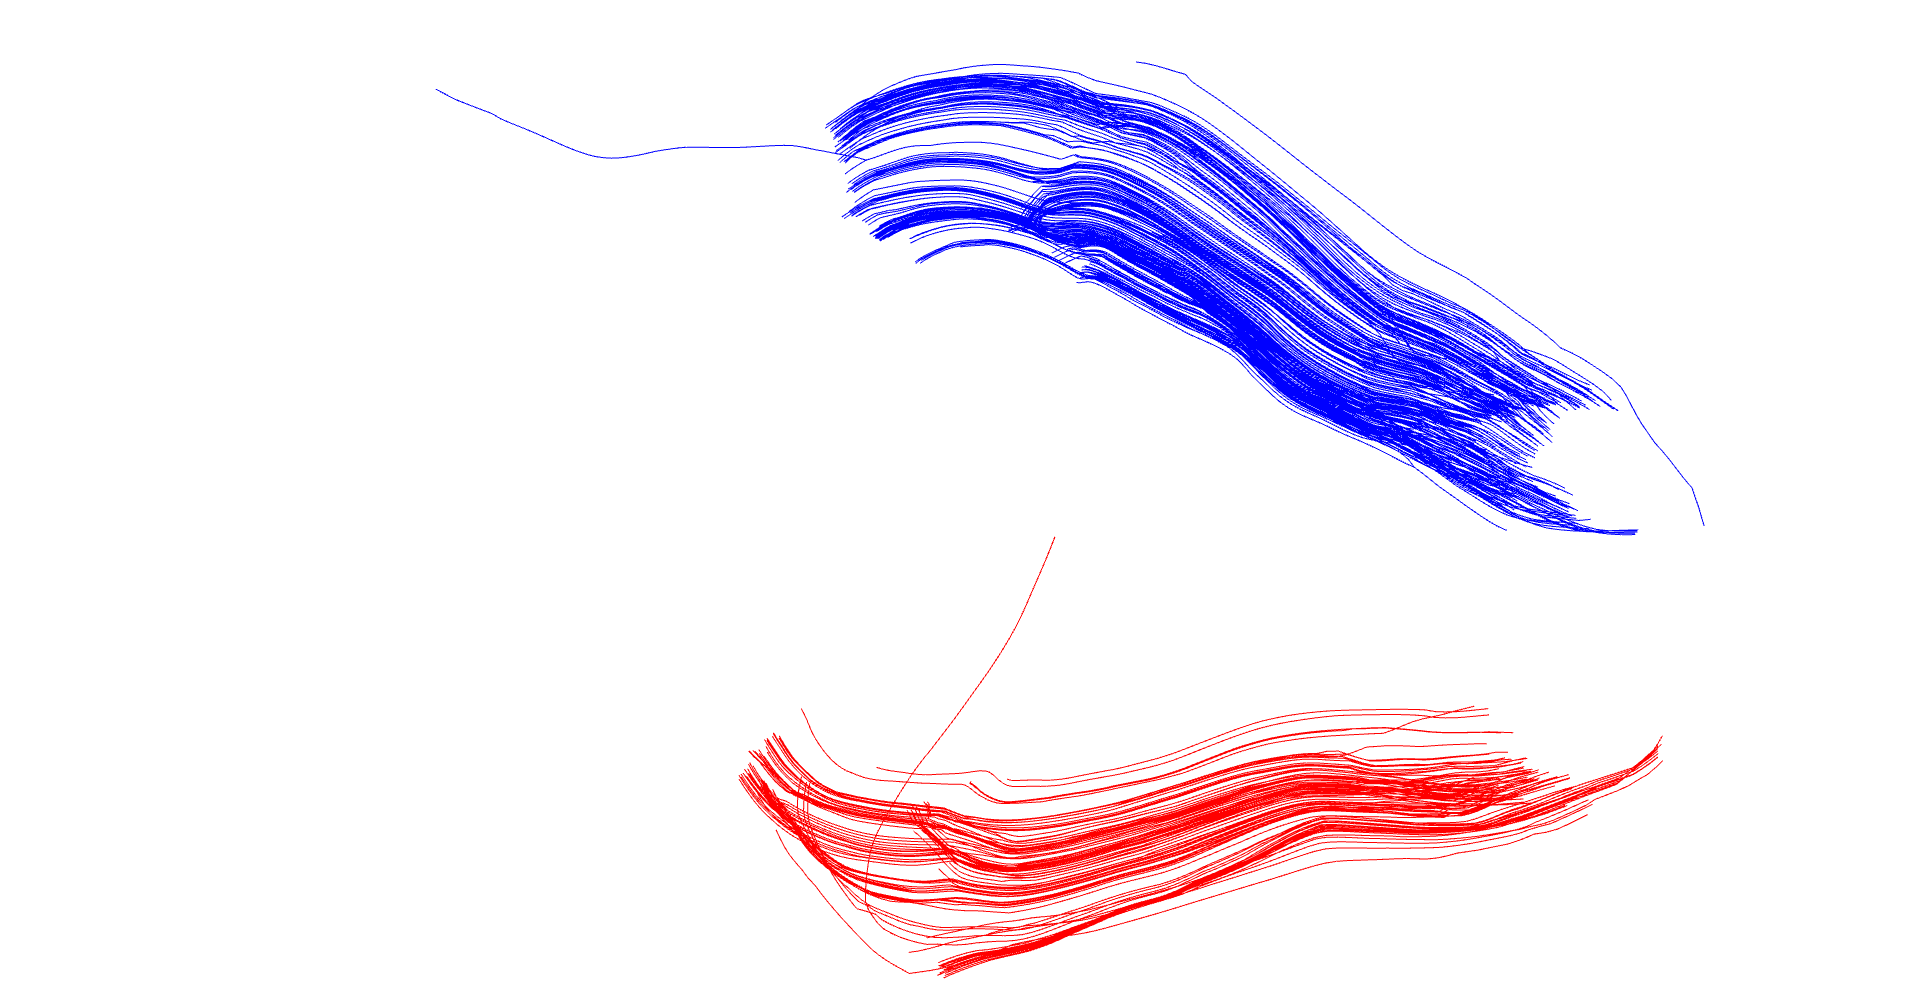
\includegraphics[scale=.7]{101_img_original}
\captionsetup{justification=centering}
\caption{The original orientation of ATR}%
{ left side (red) as target bundle and right side of ATR (blue) as template bundle}
\label{fig:img_original}
\end{figure}

\begin{figure}[H]
\centering
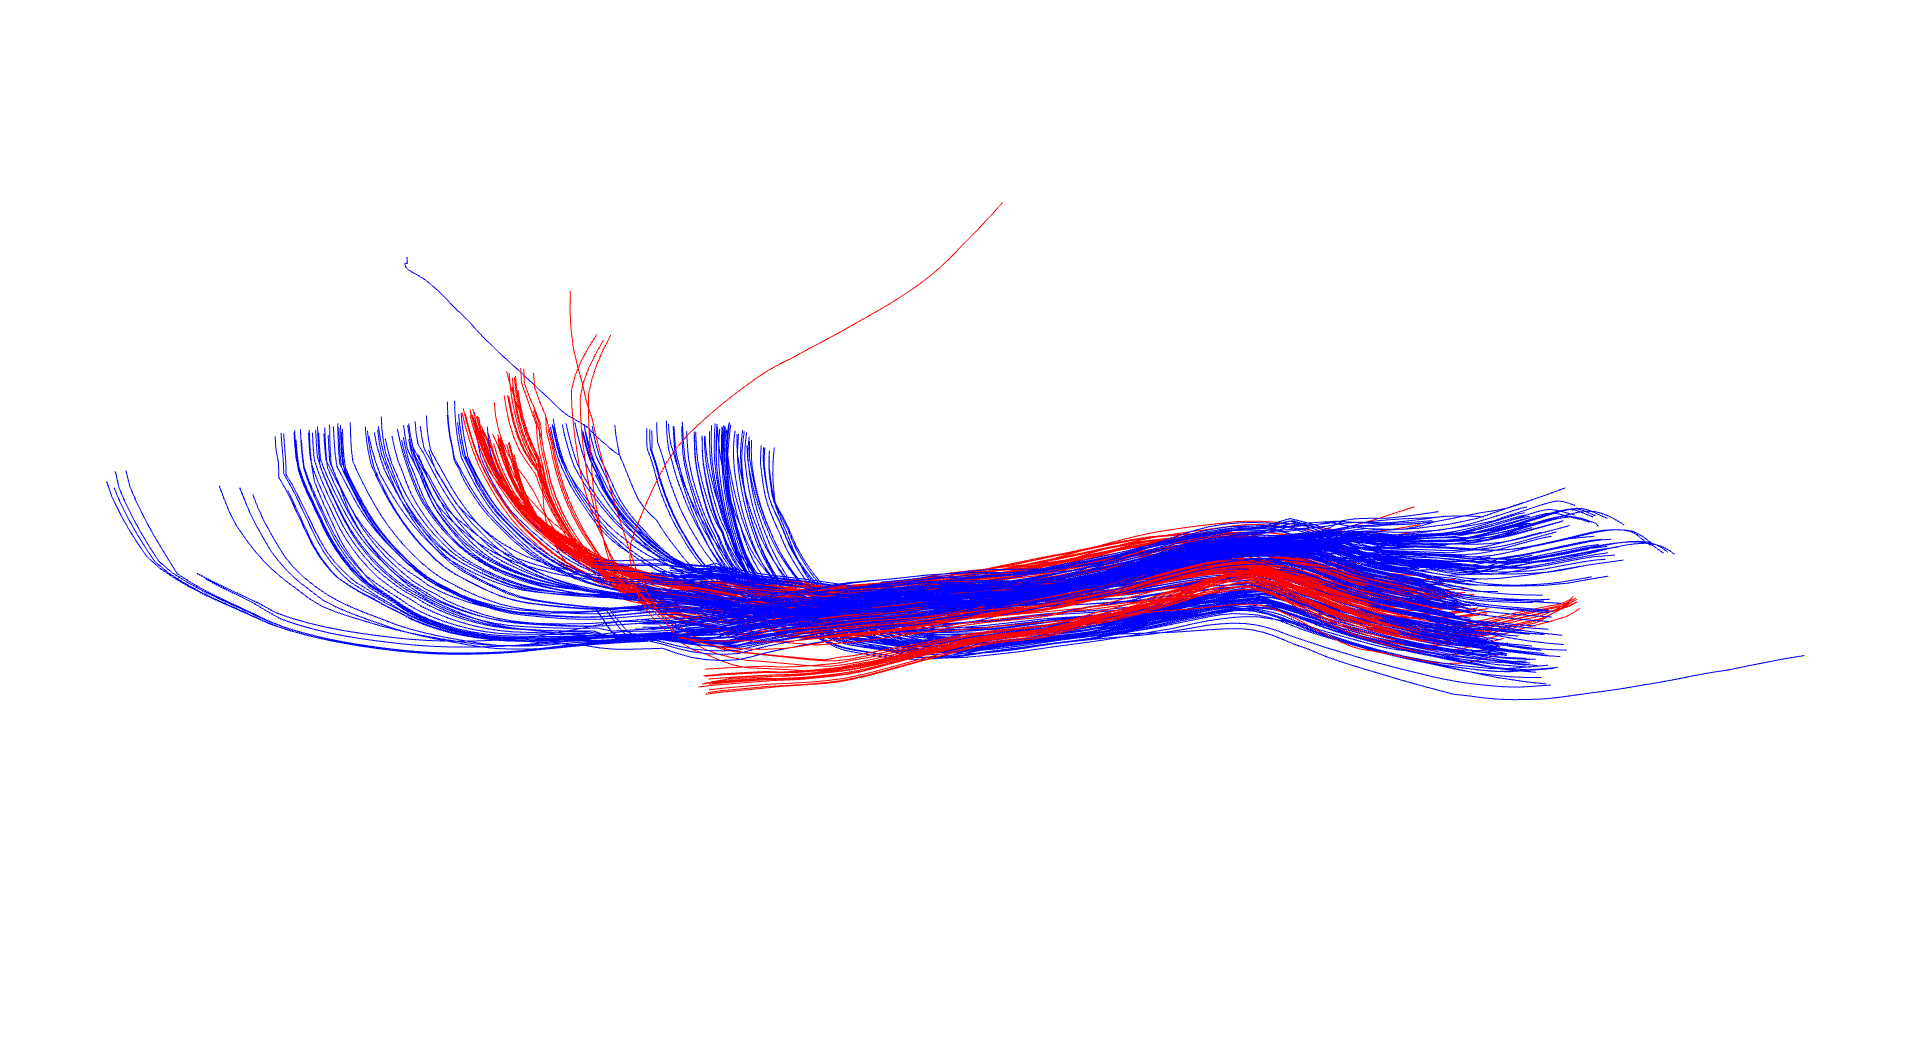
\includegraphics[scale=.3]{101_img_PCA}
\captionsetup{justification=centering}
\caption{The PCA Orientation of ATR}%
{ left side (red) as target bundle and right side of ATR (blue) as template bundle after applying PCA}
\label{fig:img_PCA}
\end{figure}

\section{Result from Experiment (1)}
\hspace{2em}In this experiment we use both side of Thalamic Radiation (ATR) fiber pathway, whereas the template bundle is the ATR on the right side and the target bundle is the left side of the ATR from the same patient.

First, we read the data (left and right side of ATR) using a tool that we customized from \textit{PlyFile} package to suit our data. Then we apply PCA and visually inspect the result as shown in Figures \ref{fig:img_original} and \ref{fig:img_PCA}. If PCA improves the alignment, we consider its result, otherwise we accept the original orientation or just flip the template bundle if two bundles are from different side of the brain.

As we can see the visual result in Figure \ref{fig:img_PCA}, the PCA tool improved the alignment, it flipped the template bundle and reduced the overall distance between to pathways. If we compare the original distances histogram in Figure \ref{fig:hist_original} to distances histogram after PCA in Figure \ref{fig:hist_PCA}, we can see the distances reduction clearly, so depending on the result we have, we consider the initial alignment for the next step (registration).

The next step is choosing the threshold, which determines the values of the weight matrix $W$ as discussed in the chapter \textit{Methods and Implementation}. The value  is \textit{one} if the distance between pint in template bundle and the correspondent point in target bundle is less than the threshold, otherwise it is \textit{one}. 

To choose the threshold we need to know the frequency of distances, therefore, we generate a histogram as shown in Figure \ref{fig:hist_PCA}. This experiment we decide to choose the value of the threshold to be seven, in this case, around ninety eight percent 98\% of points will have weight equal \textit{one} in the weight matrix $W$ and the remaining will be \textit{zeros}.

Now we need to choose the stiffness weight $\alpha$, which is not trivial, it comes after observing the visual output of the registration. If the template bundle strongly deformed and it is about to map to target bundle, then we increase the value of $\alpha$ and vice versa. In this experiment we decide the optimal value of $\alpha$ is 9999.

After we have the initial alignment using PCA and the parameters values ($\alpha$ and the threshold), we register two bundles (template and target) using ICP tool and then register the same bundles using DIPY registration function to compare the results. The visual results presented in Figure \ref{fig:registration} show that our tool has better registration and can deform the shape of the template bundle. It is clear that in ICP registration  deformed the shape of the template bundle (blue) to have a better alignment to the target graph (red).

\begin{figure}[H]
\centering
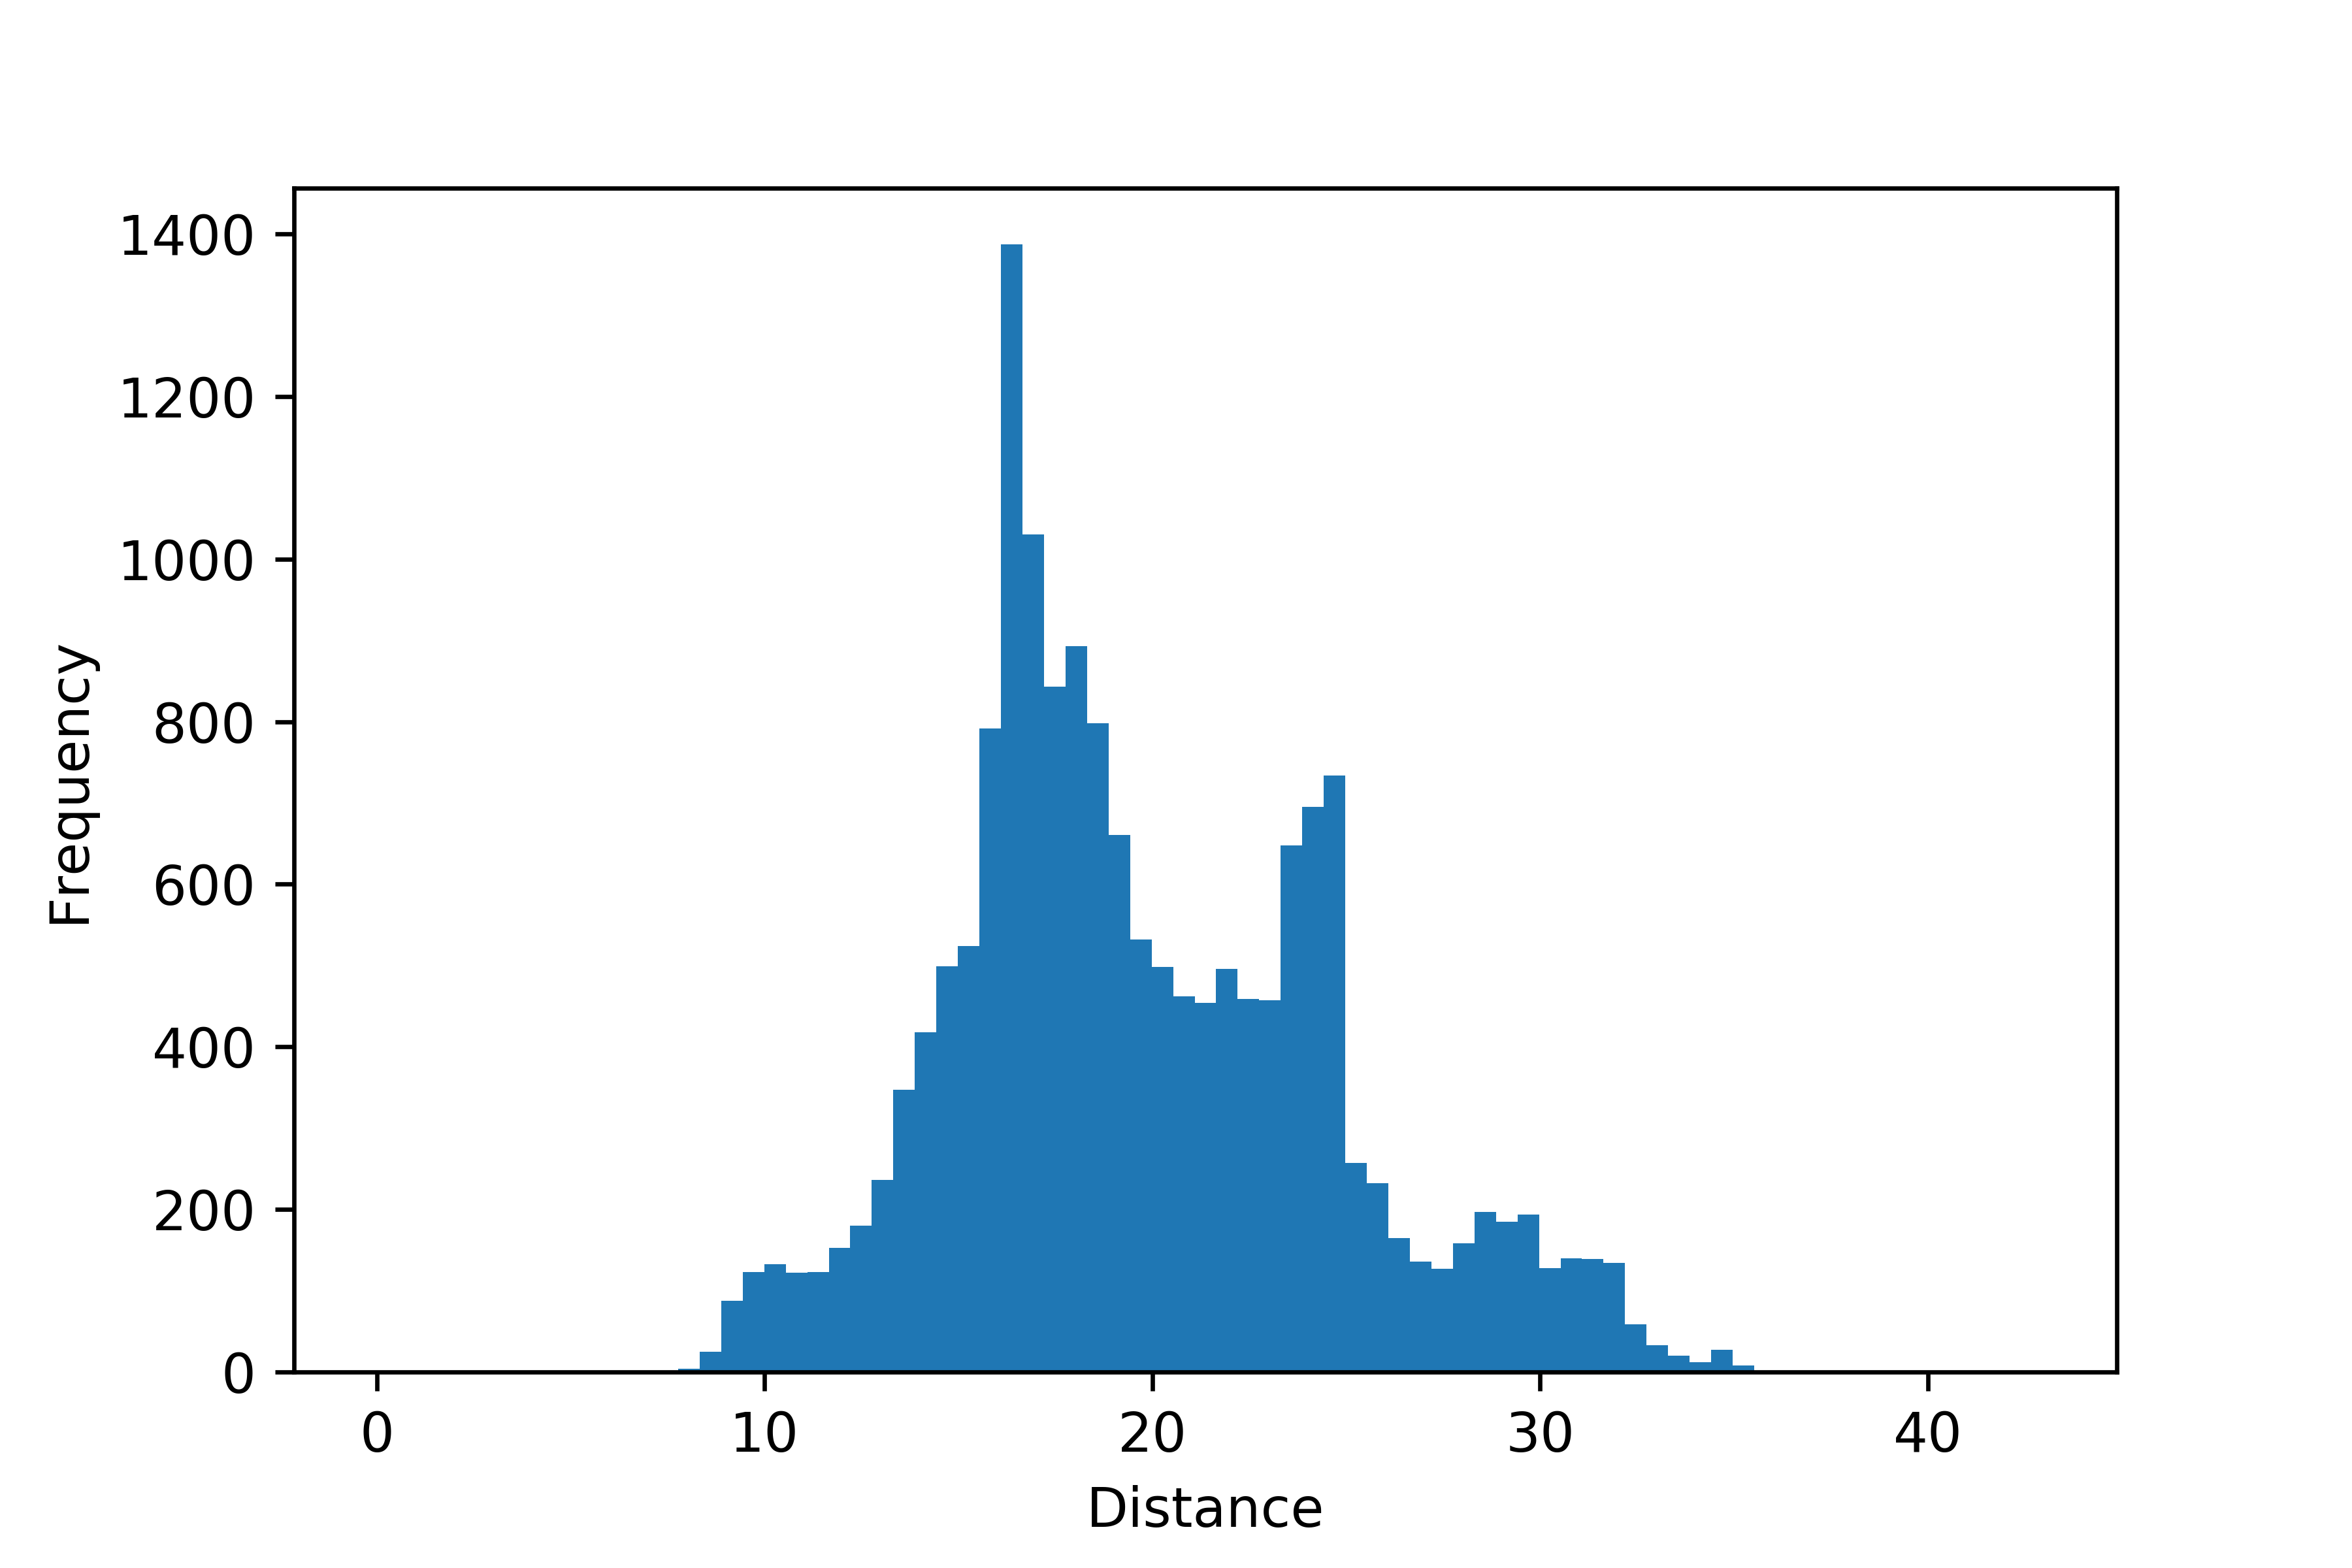
\includegraphics[scale=.90]{117_hist_original}
\captionsetup{justification=centering}
\caption{The original distances histogram of ATR}%
{The original distances histogram between ATR left and right side, it shows that the distances between points of template bundle and the points of target bundle lie between around thirty five and eight, and most of distances between fifteen and twenty five}
\label{fig:hist_original}
\end{figure}

\begin{figure}[H]
\centering
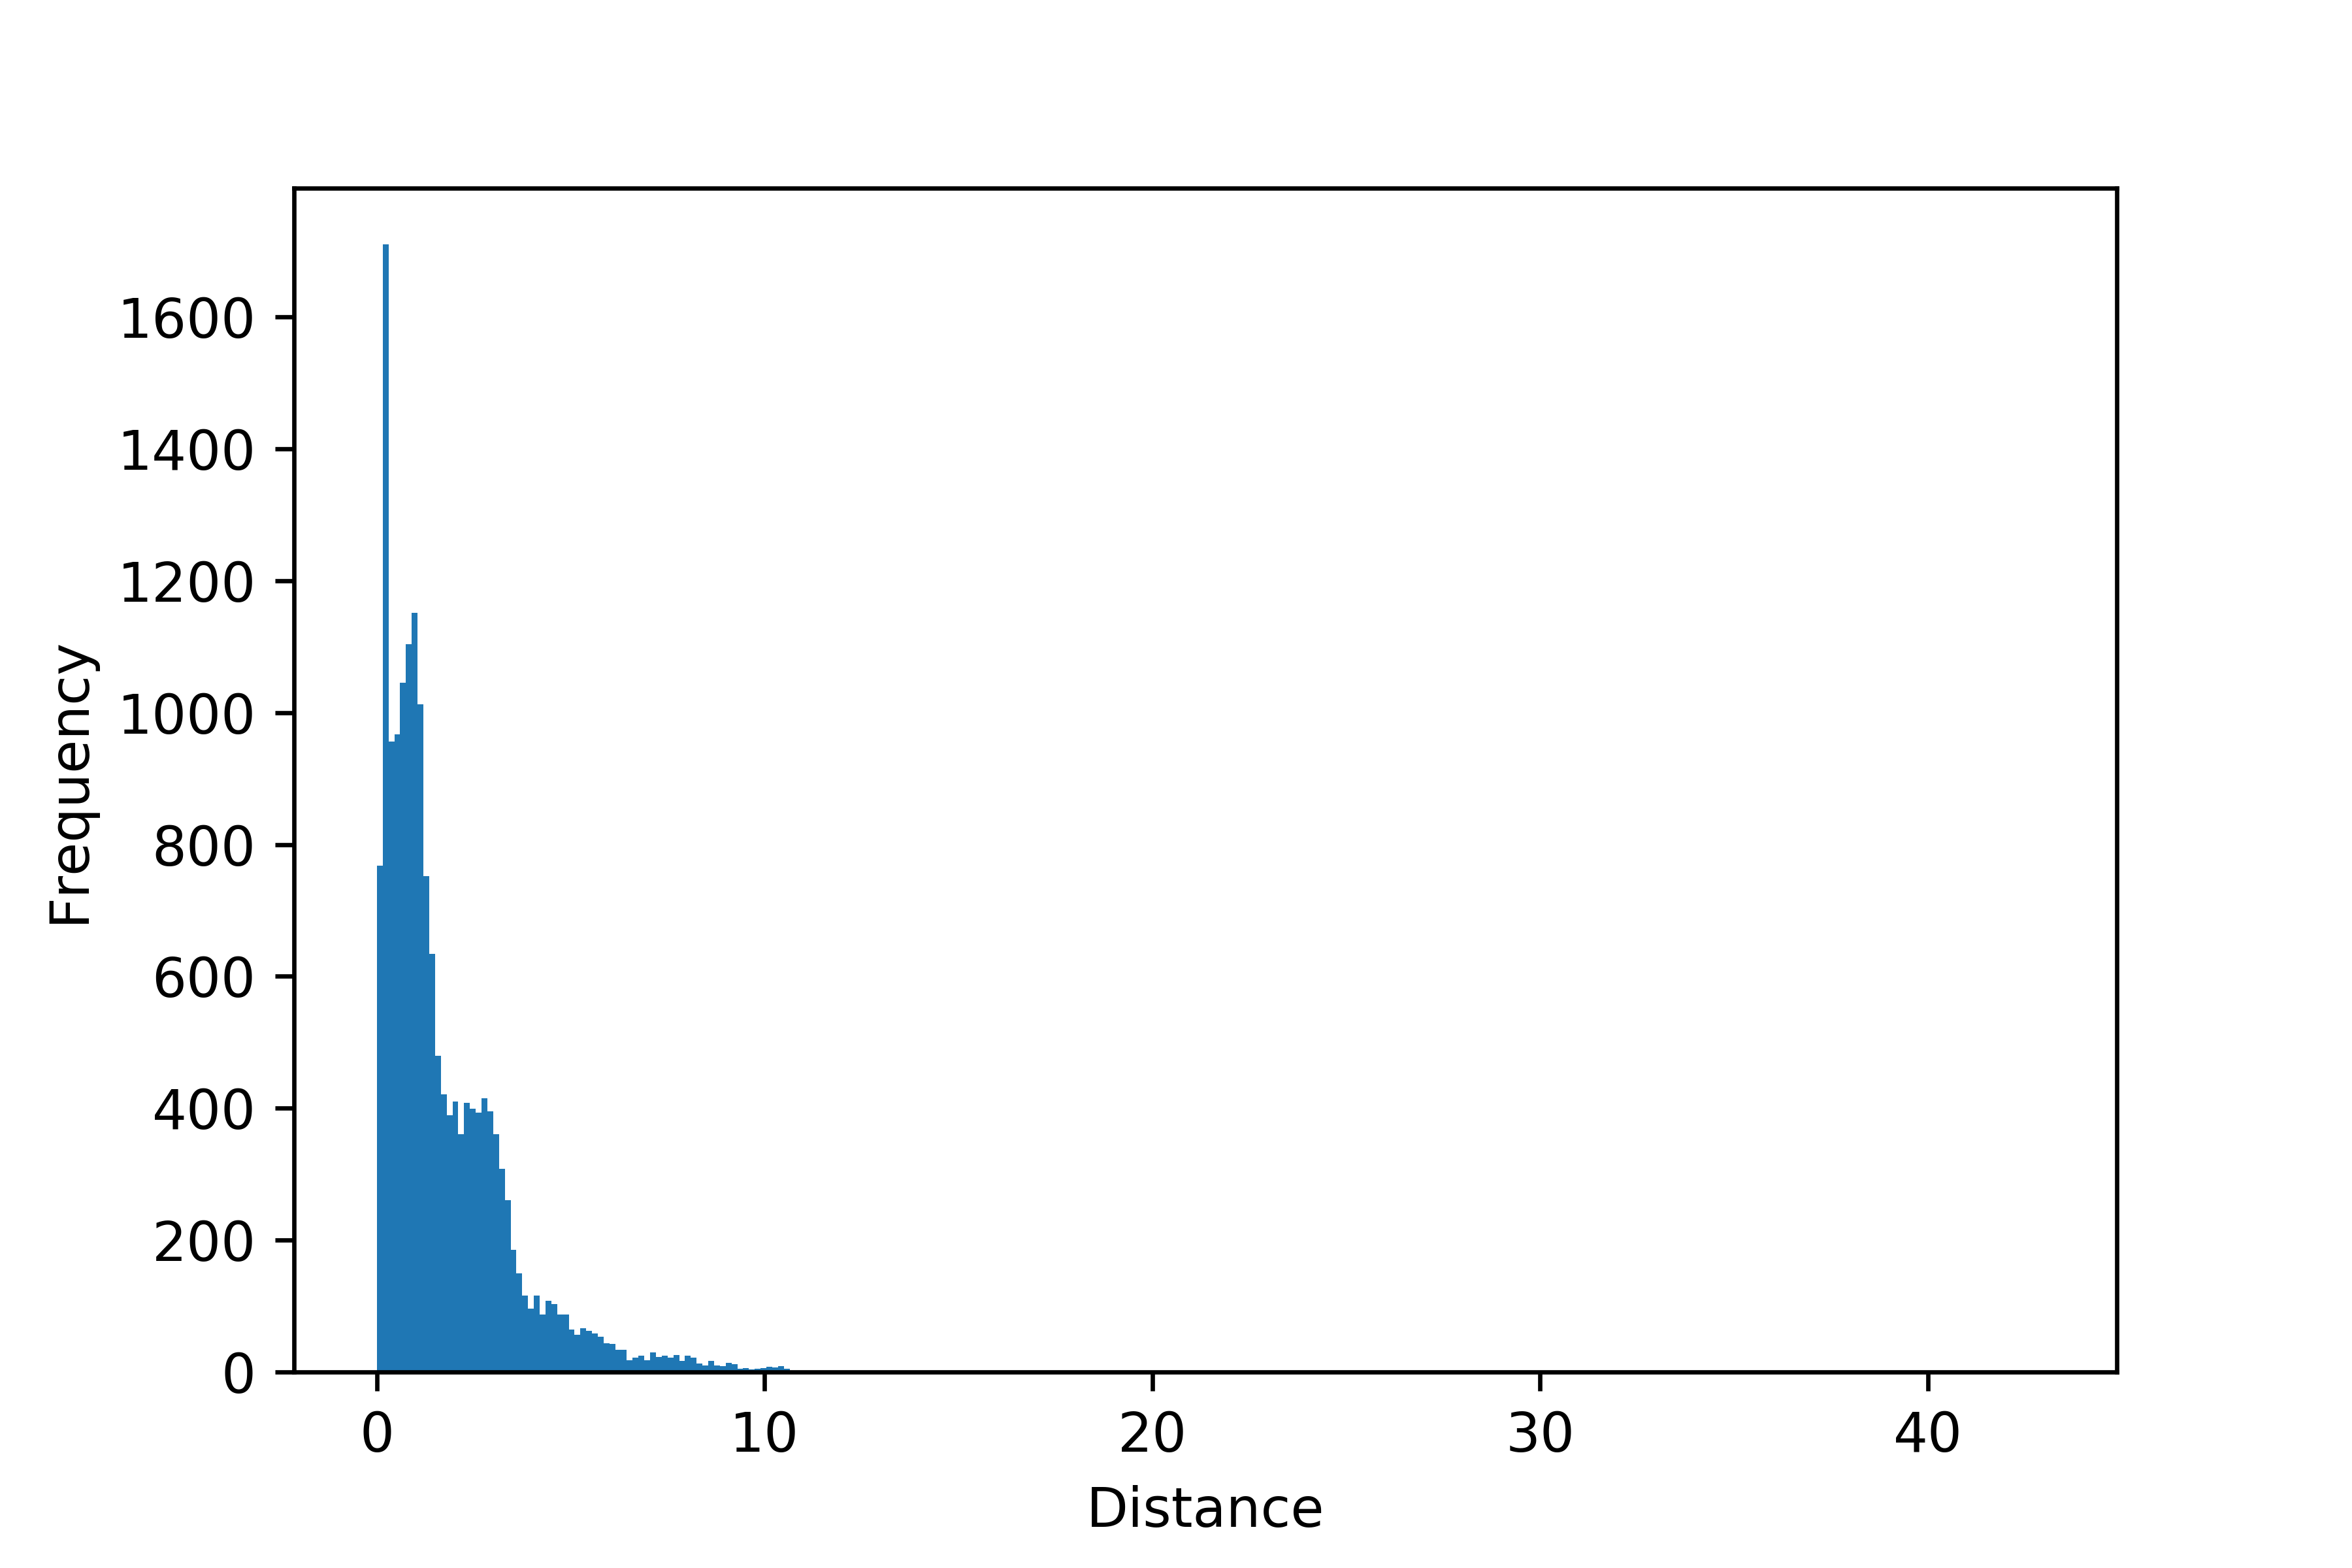
\includegraphics[scale=.90]{117_hist_PCA}
\captionsetup{justification=centering}
\caption{ATR distance Histogram after PCA}
{Distances histogram between template bundle and target bundle (ATR left and right side respectively) after applying PCA, it shows how PCA reduces the distances. Most of distances lie between zero and five}
\label{fig:hist_PCA}
\end{figure}

\begin{figure}[H]
	\centering
	\begin{subfigure}[b]{0.49\textwidth}
	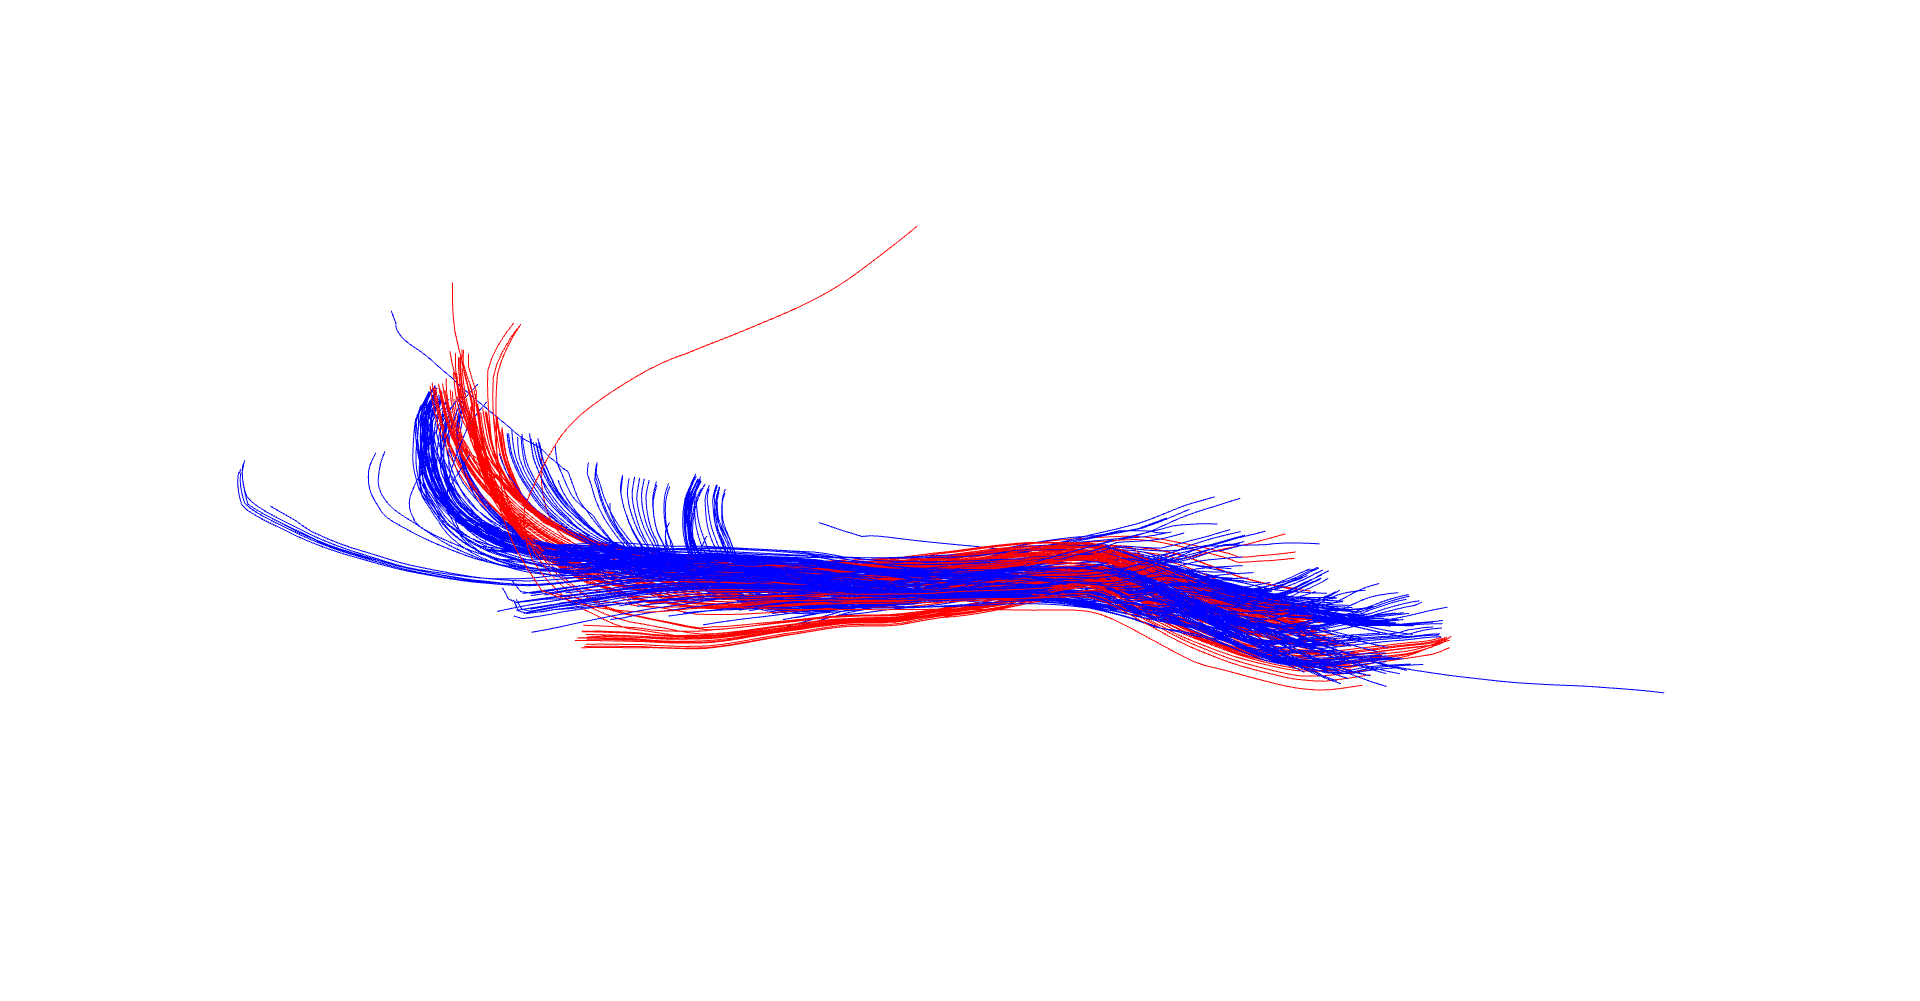
\includegraphics[width=.8\textwidth]{101_img_ICP}
	\caption{ICP registration}
	\end{subfigure}
	% separate
	\begin{subfigure}[b]{0.49\textwidth}
	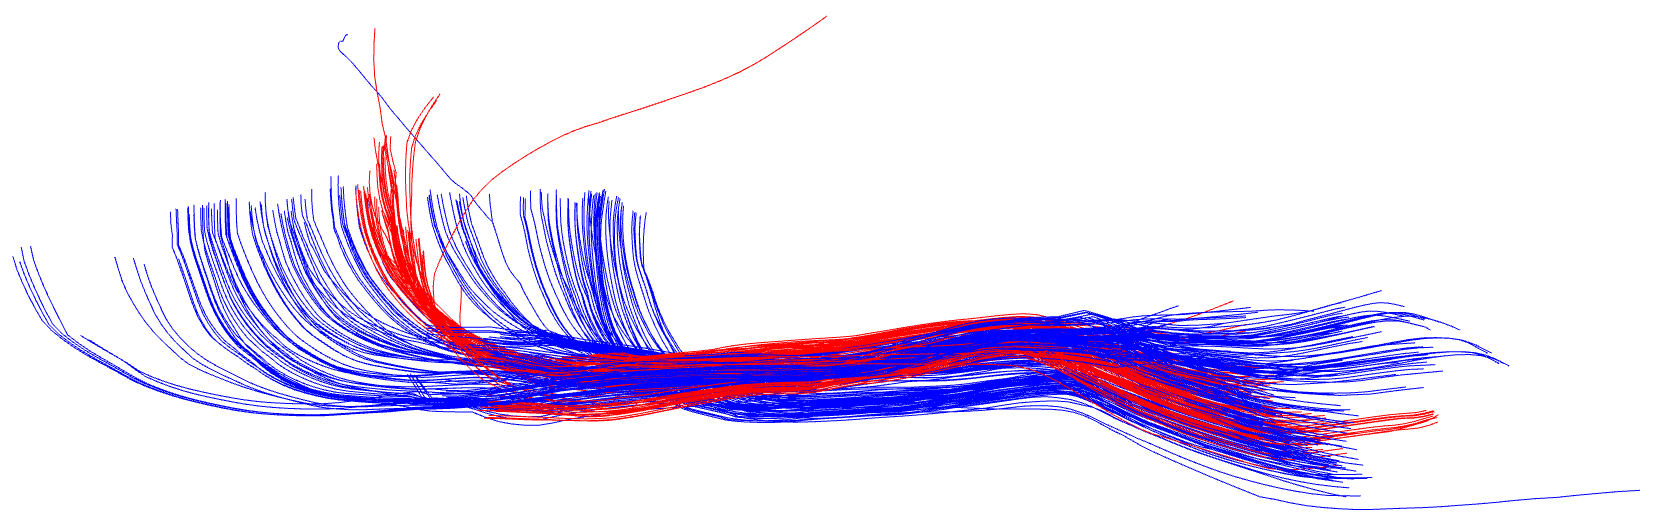
\includegraphics[width=.7\textwidth]{101_img_dipy}
	\caption{DIPY registration}
	\end{subfigure}
\caption{The Orientation after applying ICP and DIPY registration}%
{The ATR pathway left side (red) as target bundle and right side of ATR (blue) as template bundle}
\label{fig:registration}
\end{figure}

Also, we compare the distances after applying ICP and DIPY. To do so, we generate distances histograms for ICP and DIPY registration result separately to inspect the different between two methods. As we can see in Figure \ref{fig:hist_ICP}, ICP could reduce the distances where the maximum distance is around 2.5, whereas the distances histogram of the registration result of DYPY in Figure \ref{fig:hist_dipy} shows the maximum distance is around 10. We want to mention that LSQR function return acond equal \textbf{100000531}, which is average of tree time calculation of LSQR as we mention in the chapter \textit{Methods and Implementation}.

\begin{figure}[H]
\centering
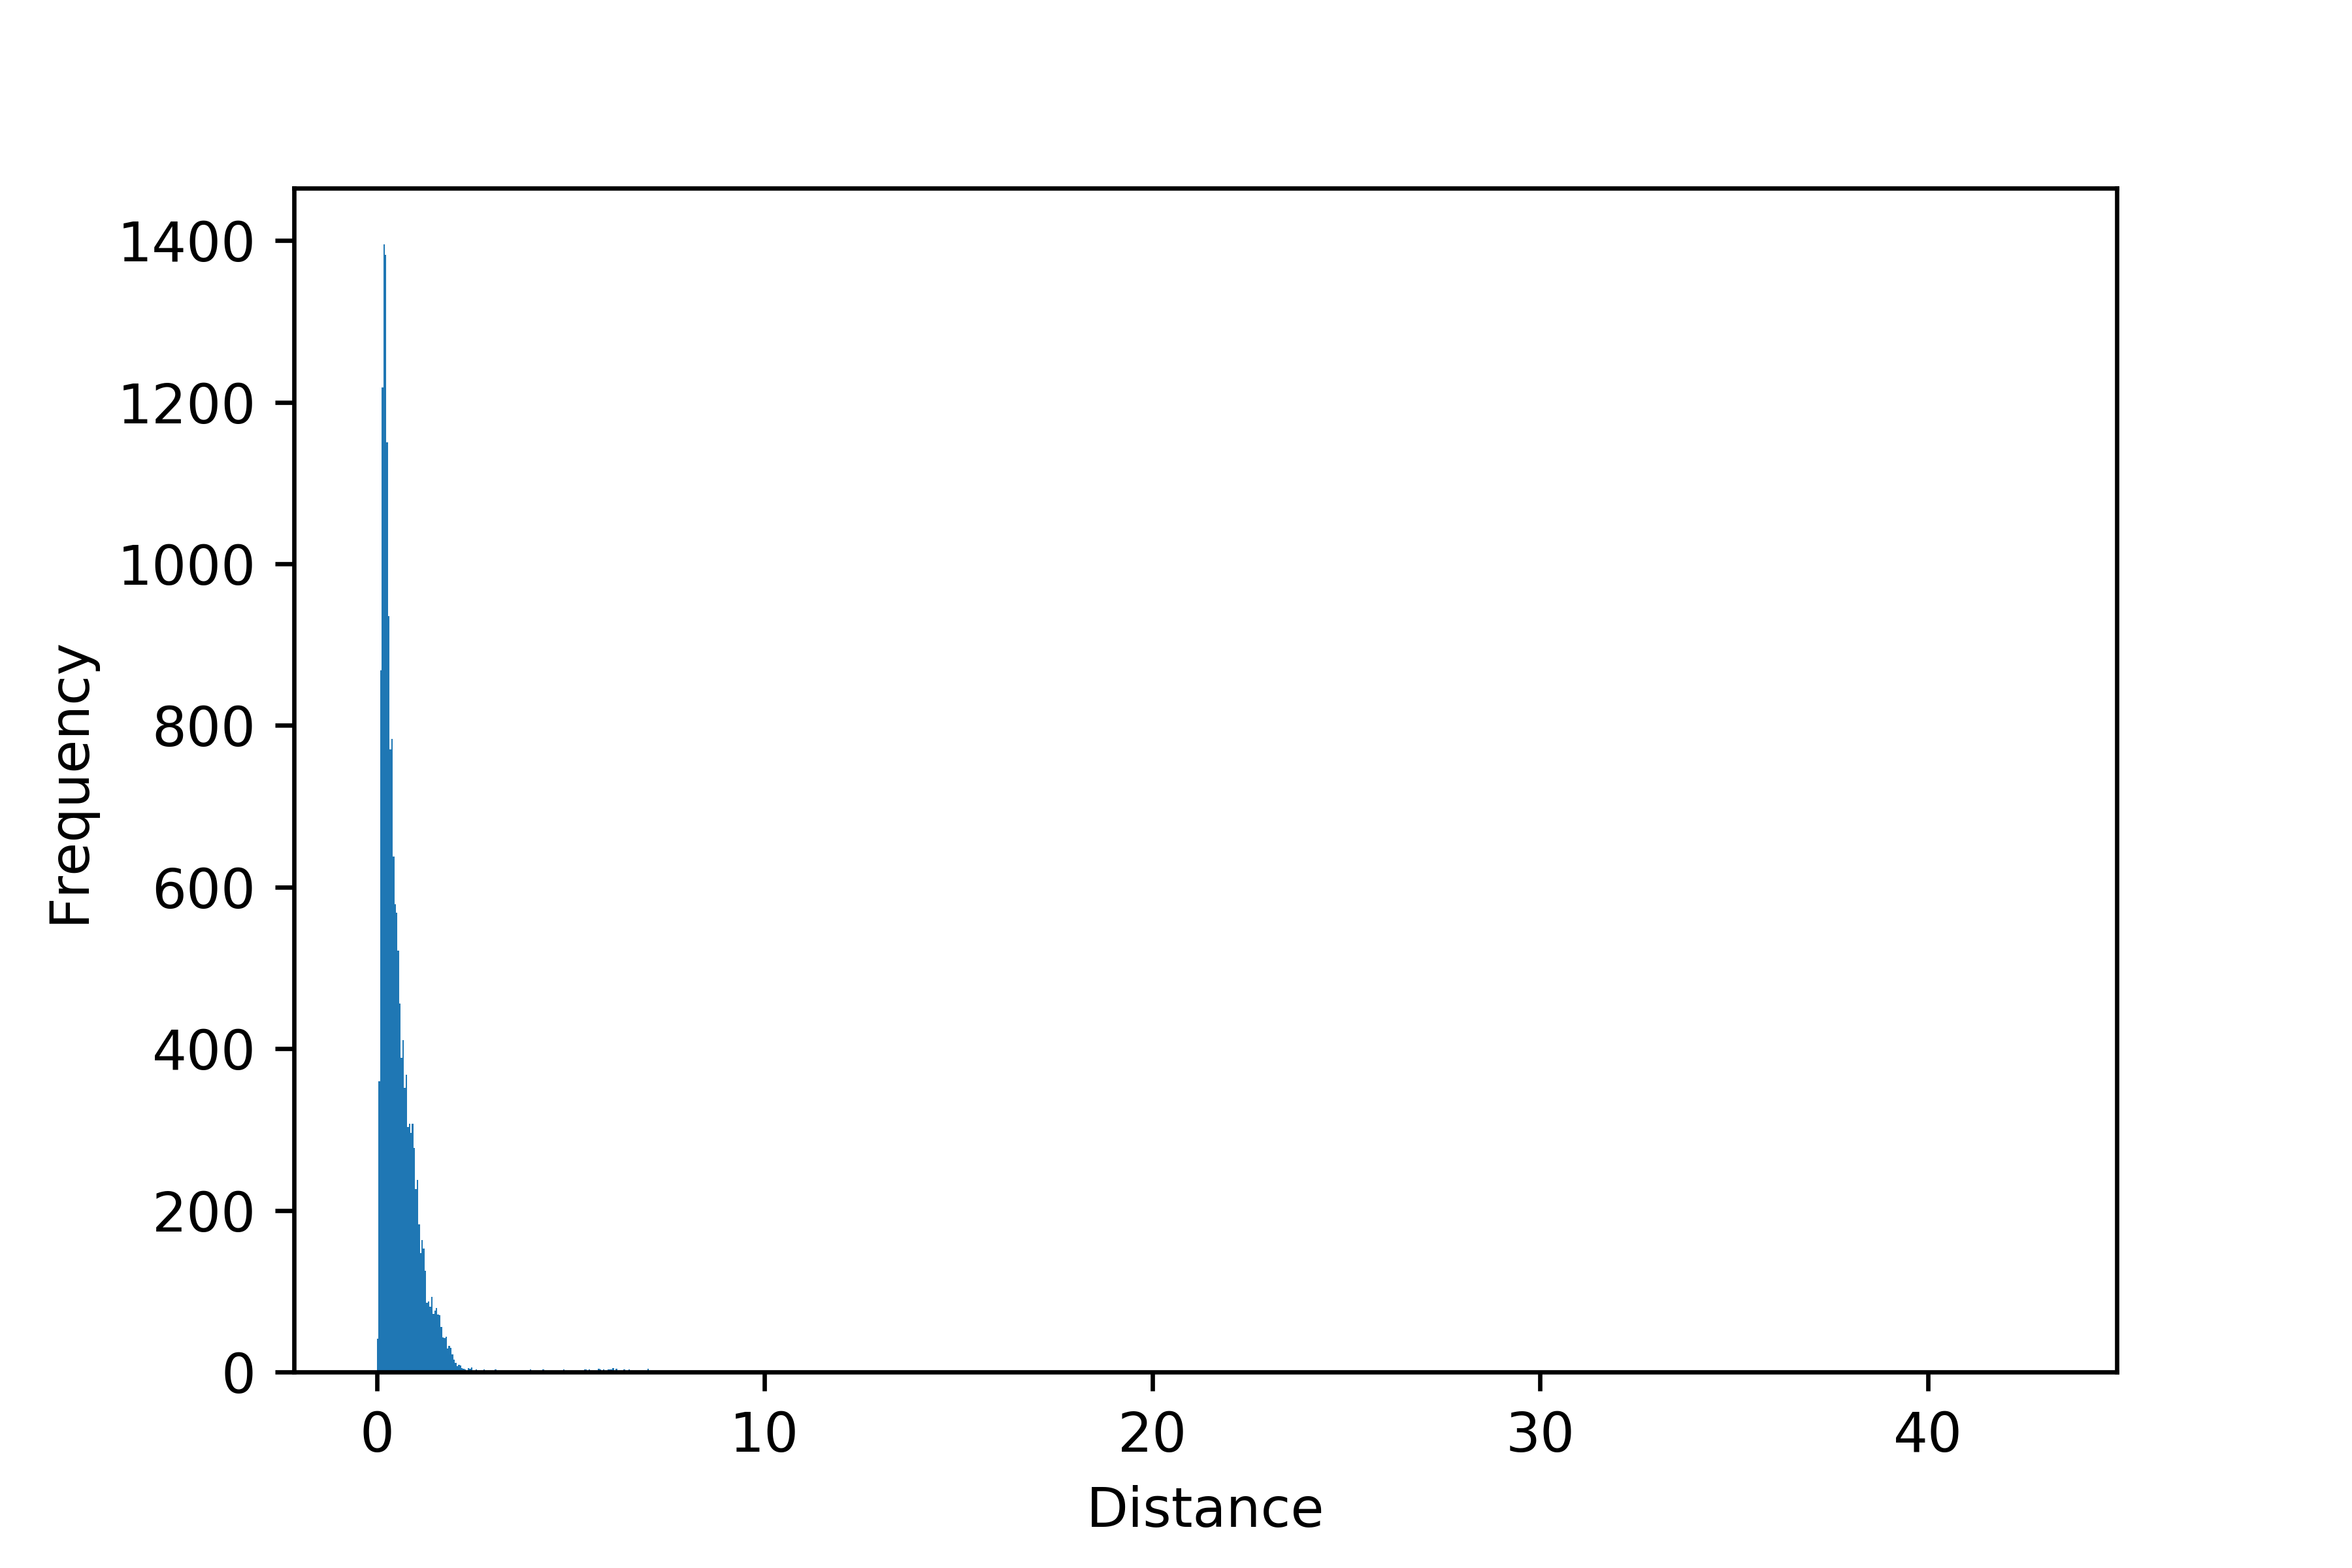
\includegraphics[scale=.90]{117_hist_ICP}
\captionsetup{justification=centering}
\caption{Distances histogram after ICP}%
{The histogram shows the frequency of distances between template points and correspondent points in target graph (ATR left and right side respectively) after applying non-rigid ICP registration.}
\label{fig:hist_ICP}
\end{figure}

\begin{figure}[H]
\centering
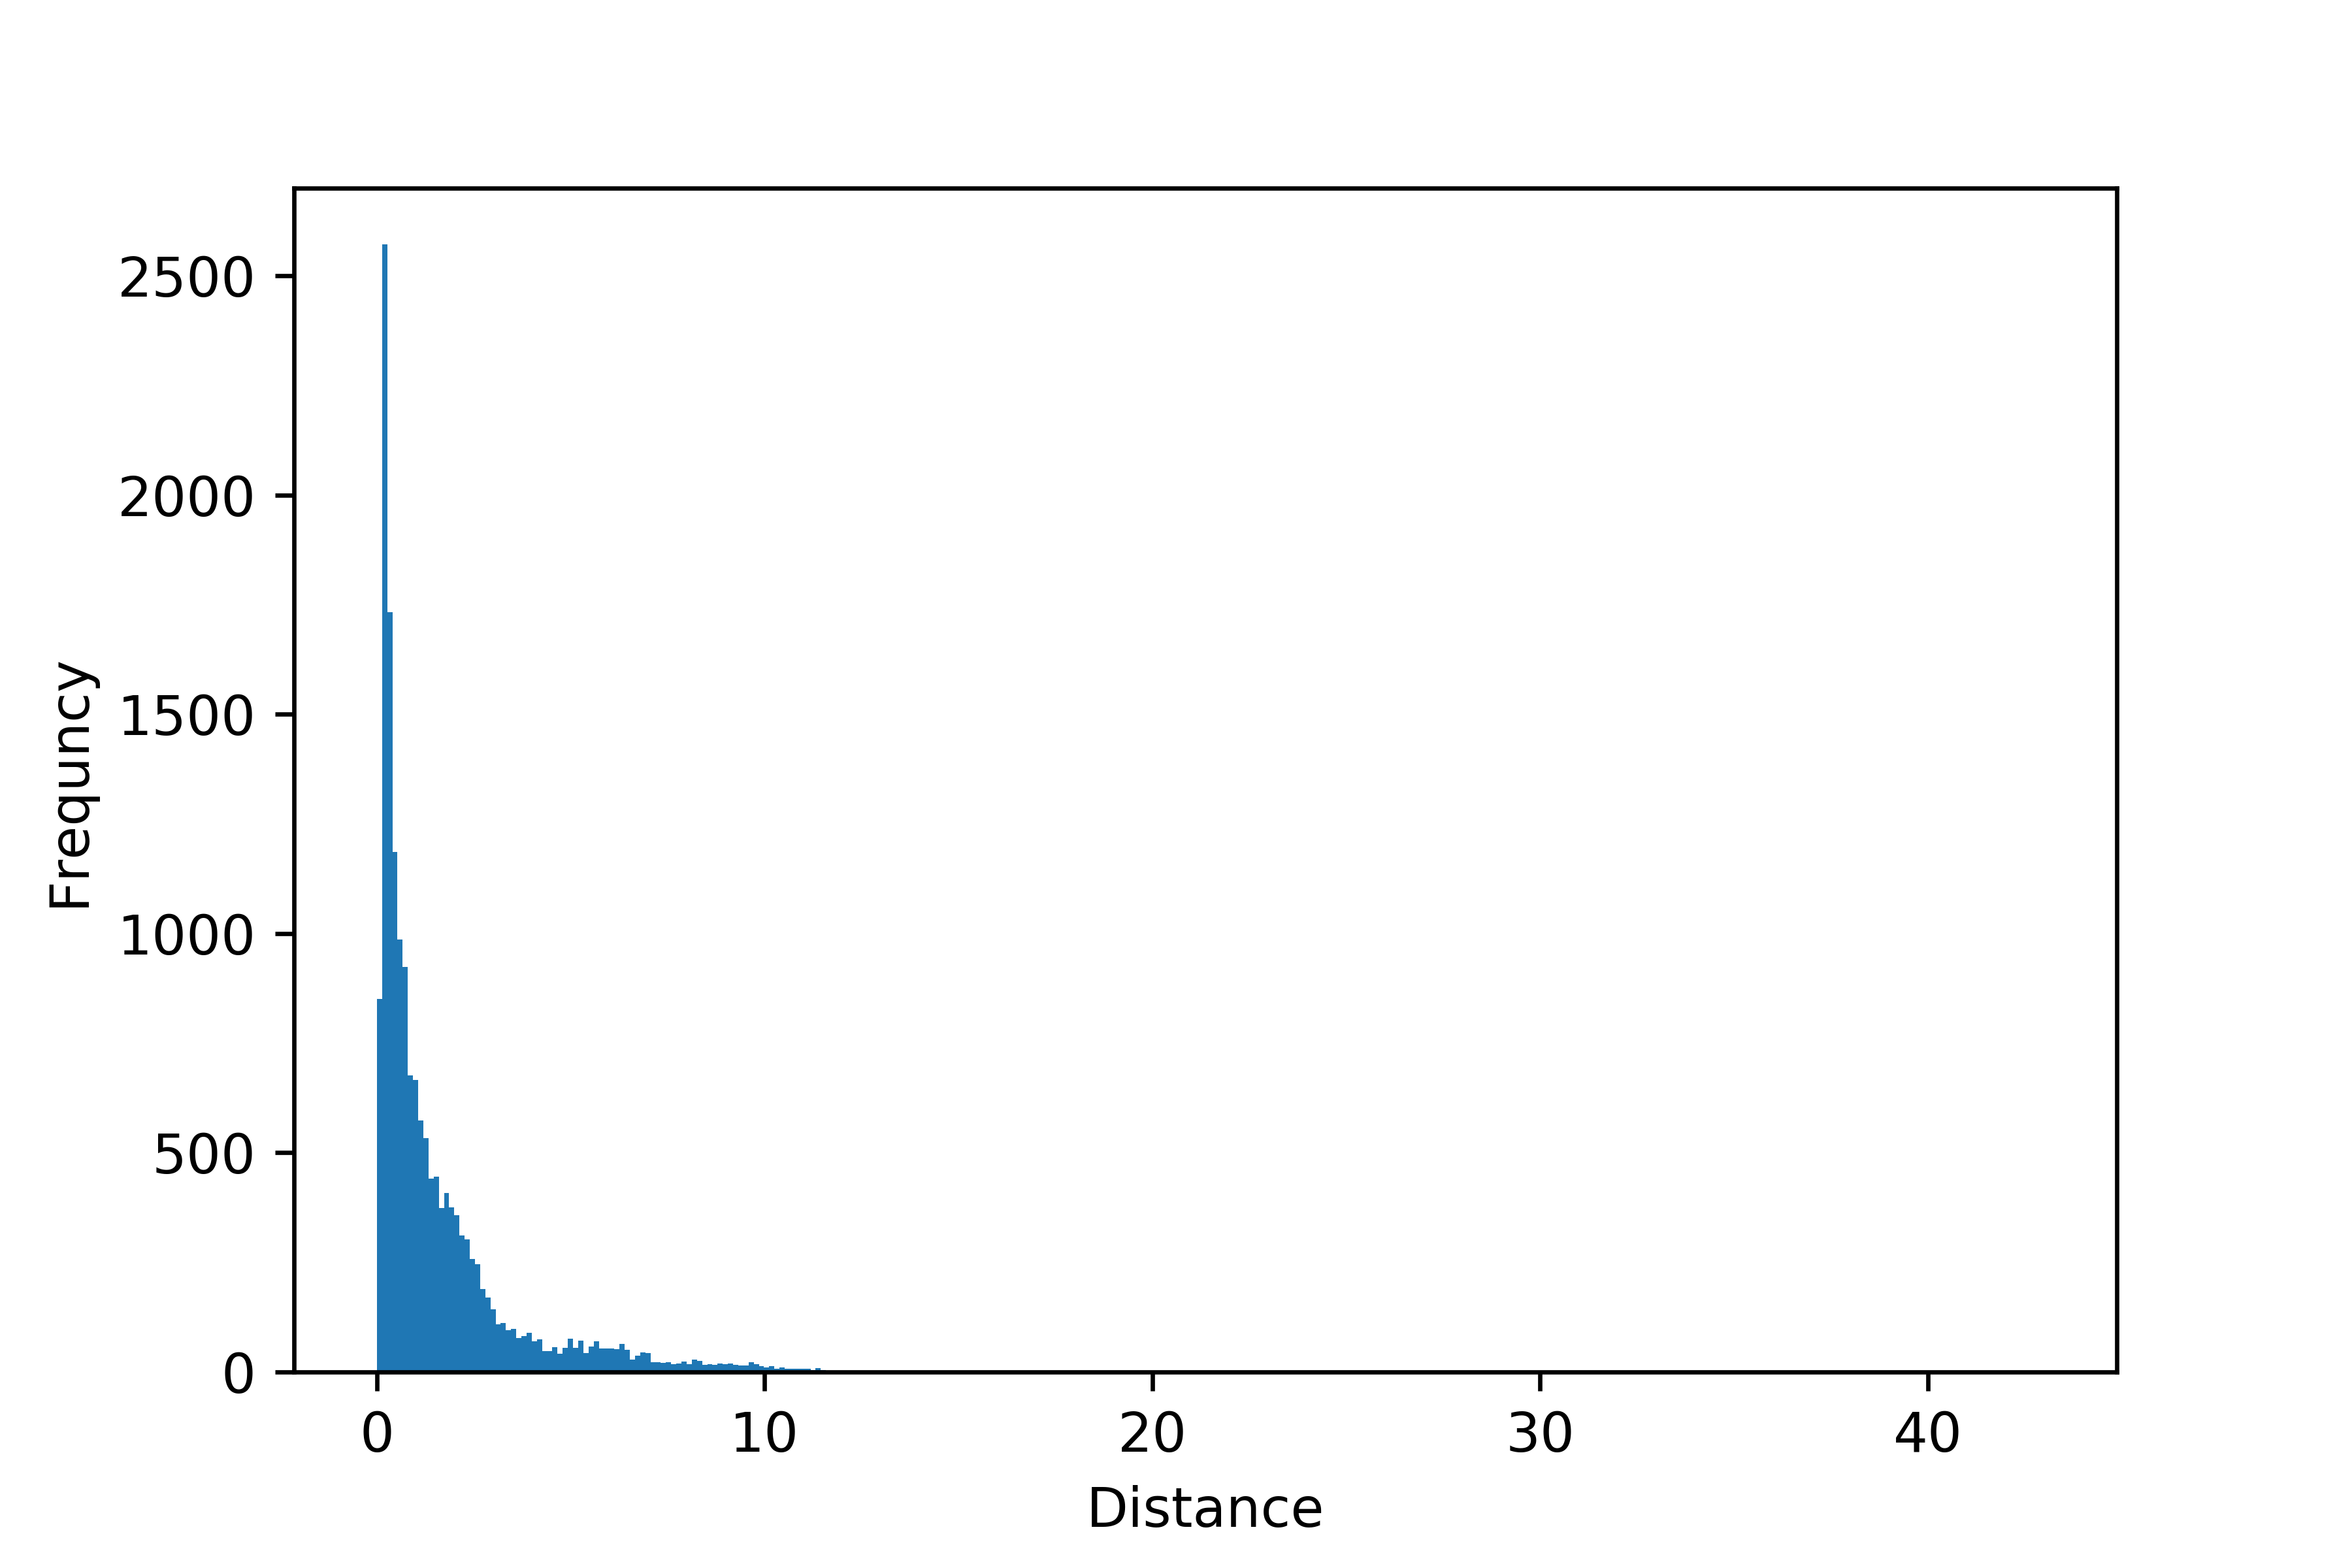
\includegraphics[scale=.90]{117_dipy_hist}
\captionsetup{justification=centering}
\caption{Distances histogram after DIPY}%
{The histogram shows the frequency of distances between template points and correspondent points in target graph (ATR left and right side respectively) after applying DIPY registration.}
\label{fig:hist_dipy}
\end{figure}

\section{Result from Experiment (2)}
The second experiment tests how the method can correct the deformation. To evaluate this, we take one pathway, deform its shape locally (local transformation) and try to correct the deformation again and get the original shape again (almost). Essentially, what we mean by local transformation is that we apply different affine transformation matrices for each point in the bundle. 

In this experiment we choose the right side of ATR and apply local transformation on it as we mentioned. Then we try to register the deformed pathway with the original one using ICP and then DIPY. As we can see in Figures \ref{fig:registration3}, non-rigid ICP can correct the deformation appropriately, whereas DIPY can give optimal alignment but it can not correct the deformation. The return value average of acond equal \textbf{5741672}

\begin{figure}[H]
\centering
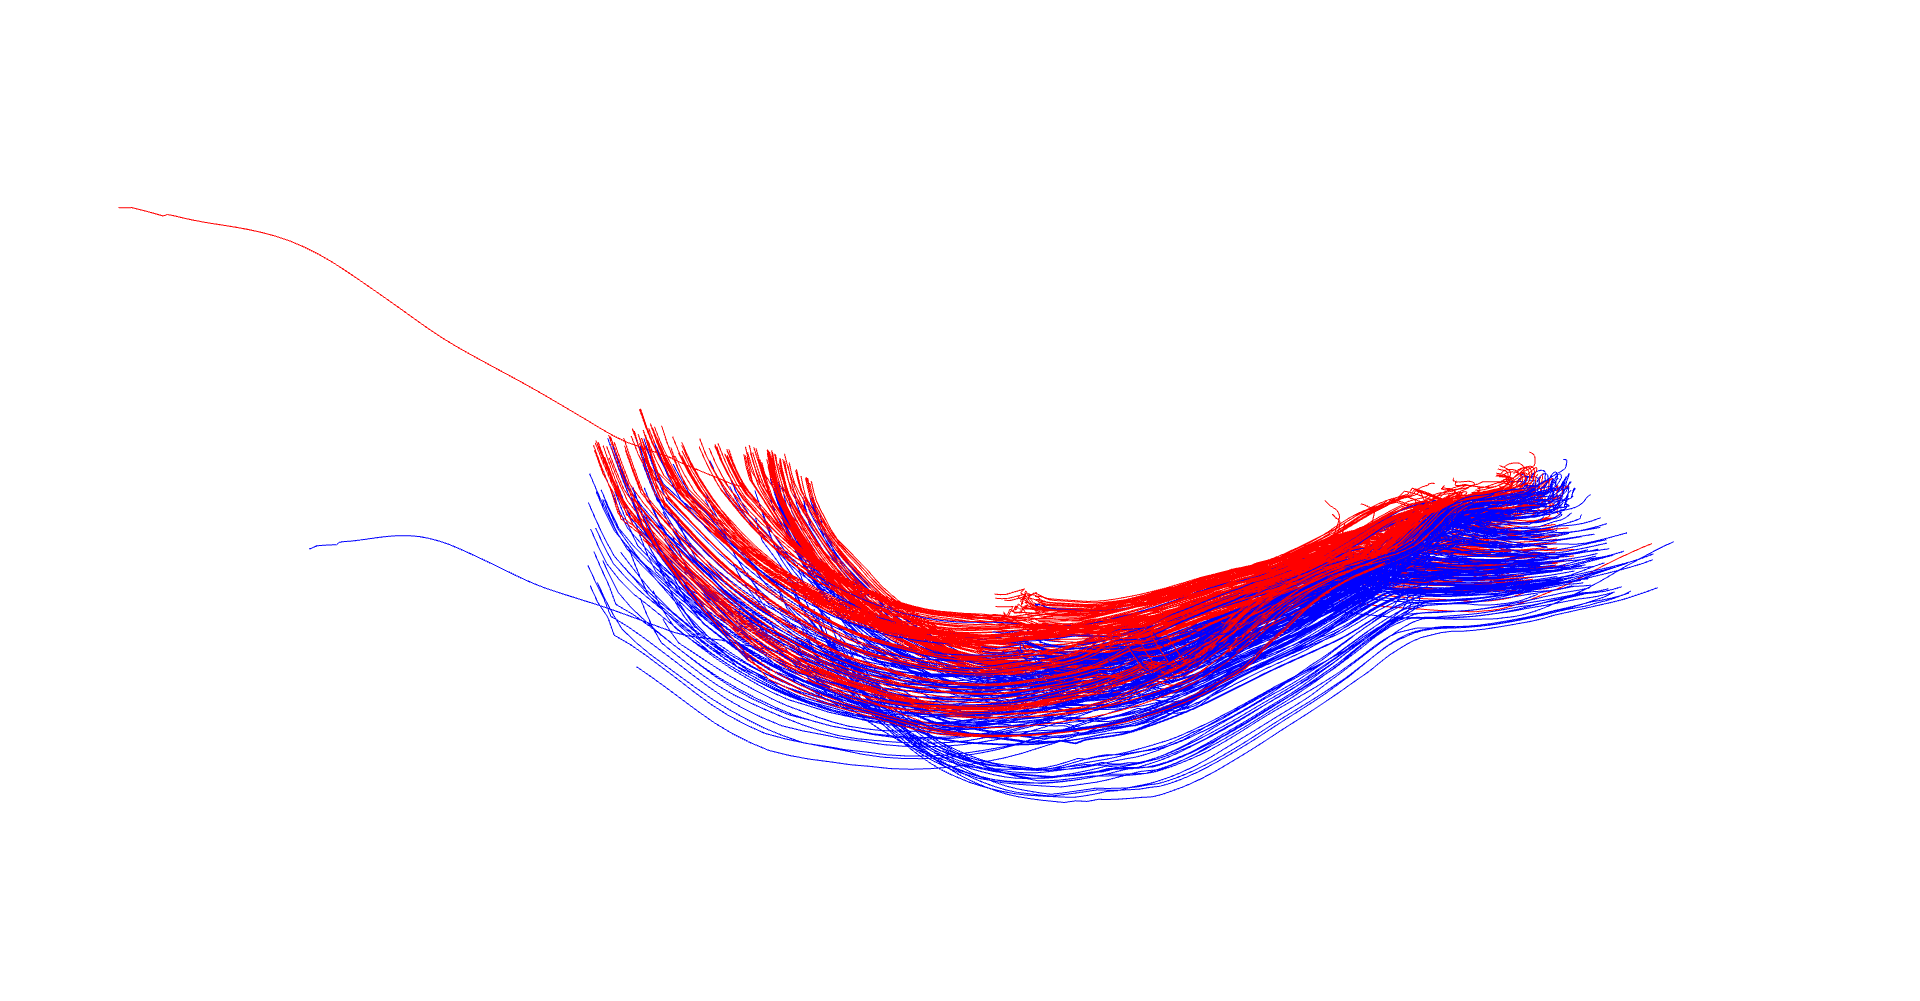
\includegraphics[scale=.30]{102_img_original}
\captionsetup{justification=centering}
\caption{The original visual orientation}%
{The orientation of ATR left side before deformation (the original pathway (red)) and after local deformation (blue). This orientation consider as the original orientation before registration}
\label{fig:img_original_def}
\end{figure}

\begin{figure}[H]
	\centering
	\begin{subfigure}[b]{0.49\textwidth}
	\centering
	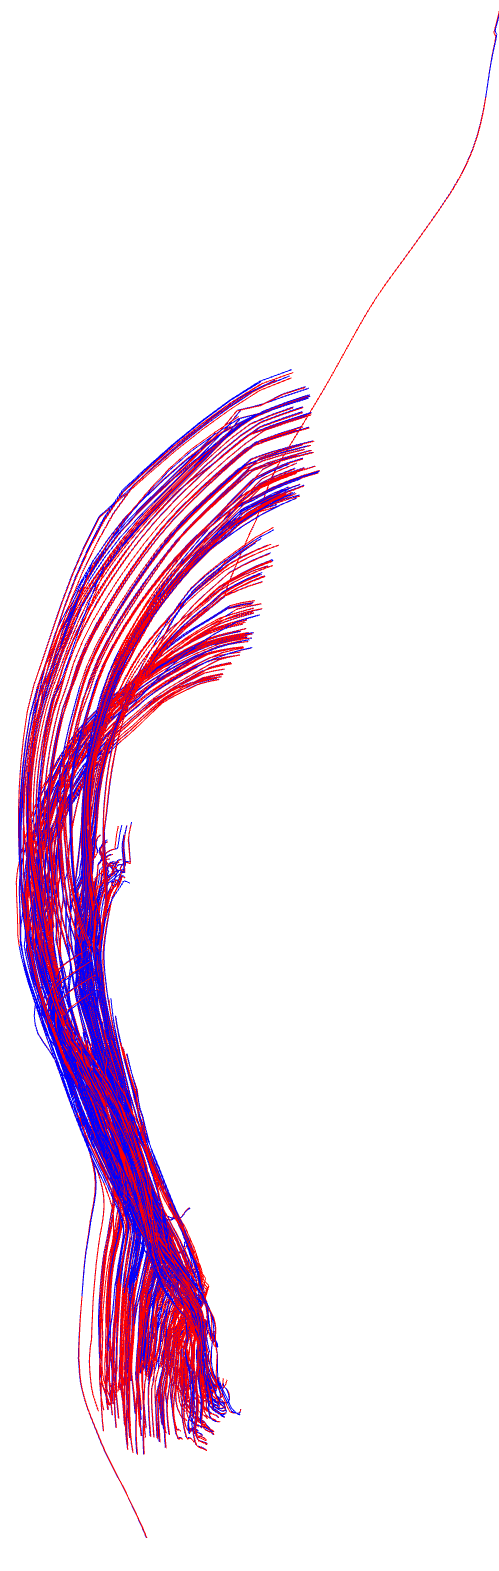
\includegraphics[width=.5\textwidth]{102_img_ICP}
	\caption{Orientation after ICP registration}
	\end{subfigure}
	% separate
	\begin{subfigure}[b]{0.49\textwidth}
	\centering
	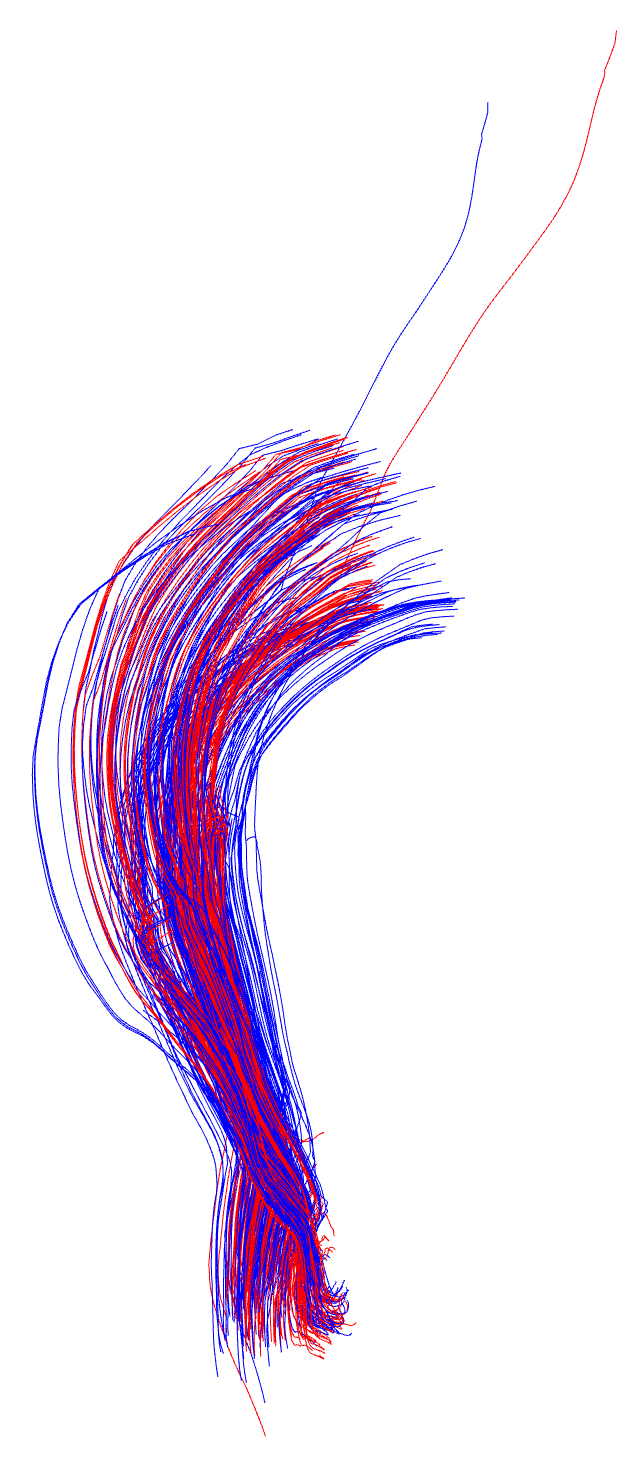
\includegraphics[width=.7\textwidth]{102_img_dipy}
	\caption{Orientation after DIPY registration}
	\end{subfigure}
\captionsetup{justification=centering}
\caption{Visual orientation after registration}
{The orientation of ATR left side before deformation (red) and after local deformation (blue).}
\label{fig:registration3}
\end{figure}

\begin{figure}[H]
\centering
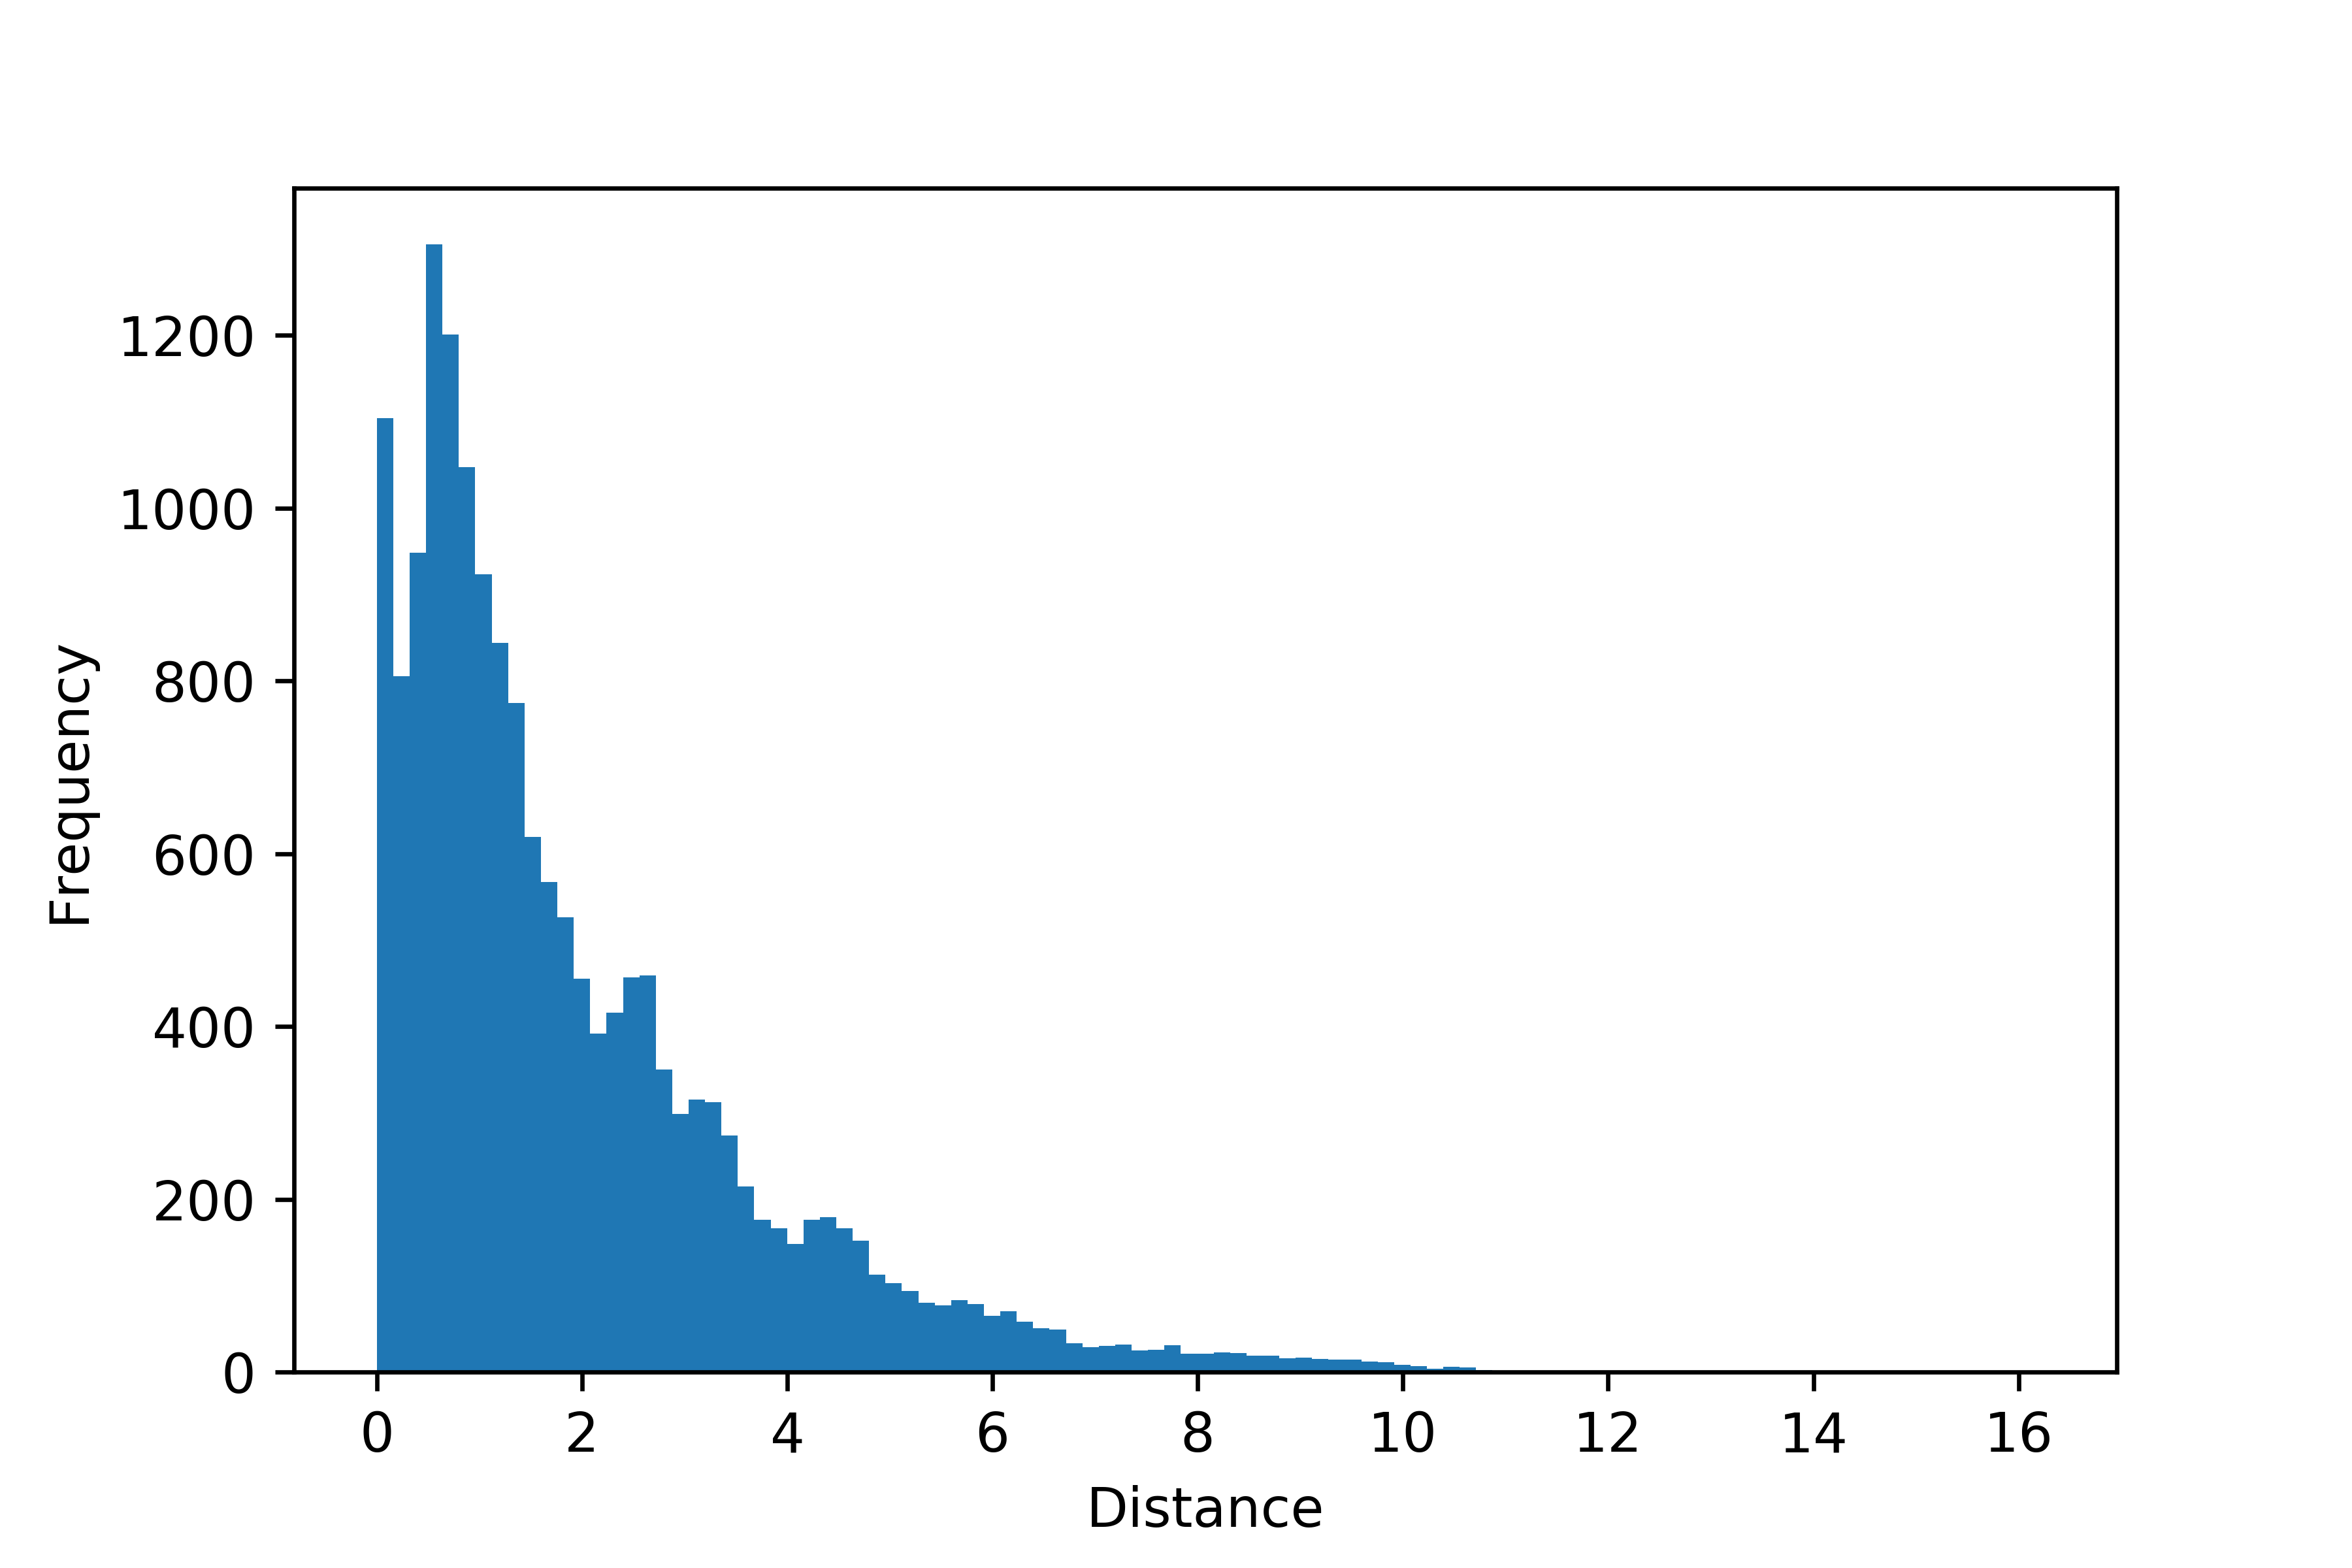
\includegraphics[scale=.7]{118_hist_original}
\captionsetup{justification=centering}
\caption{Original deformed bundle distances histogram}
{The histogram shows the frequency of distances between the original pathway points (before local deformation) and correspondent points in the locally deformed version.}
\label{fig:hist_original_def}
\end{figure}

\begin{figure}[H]
\centering
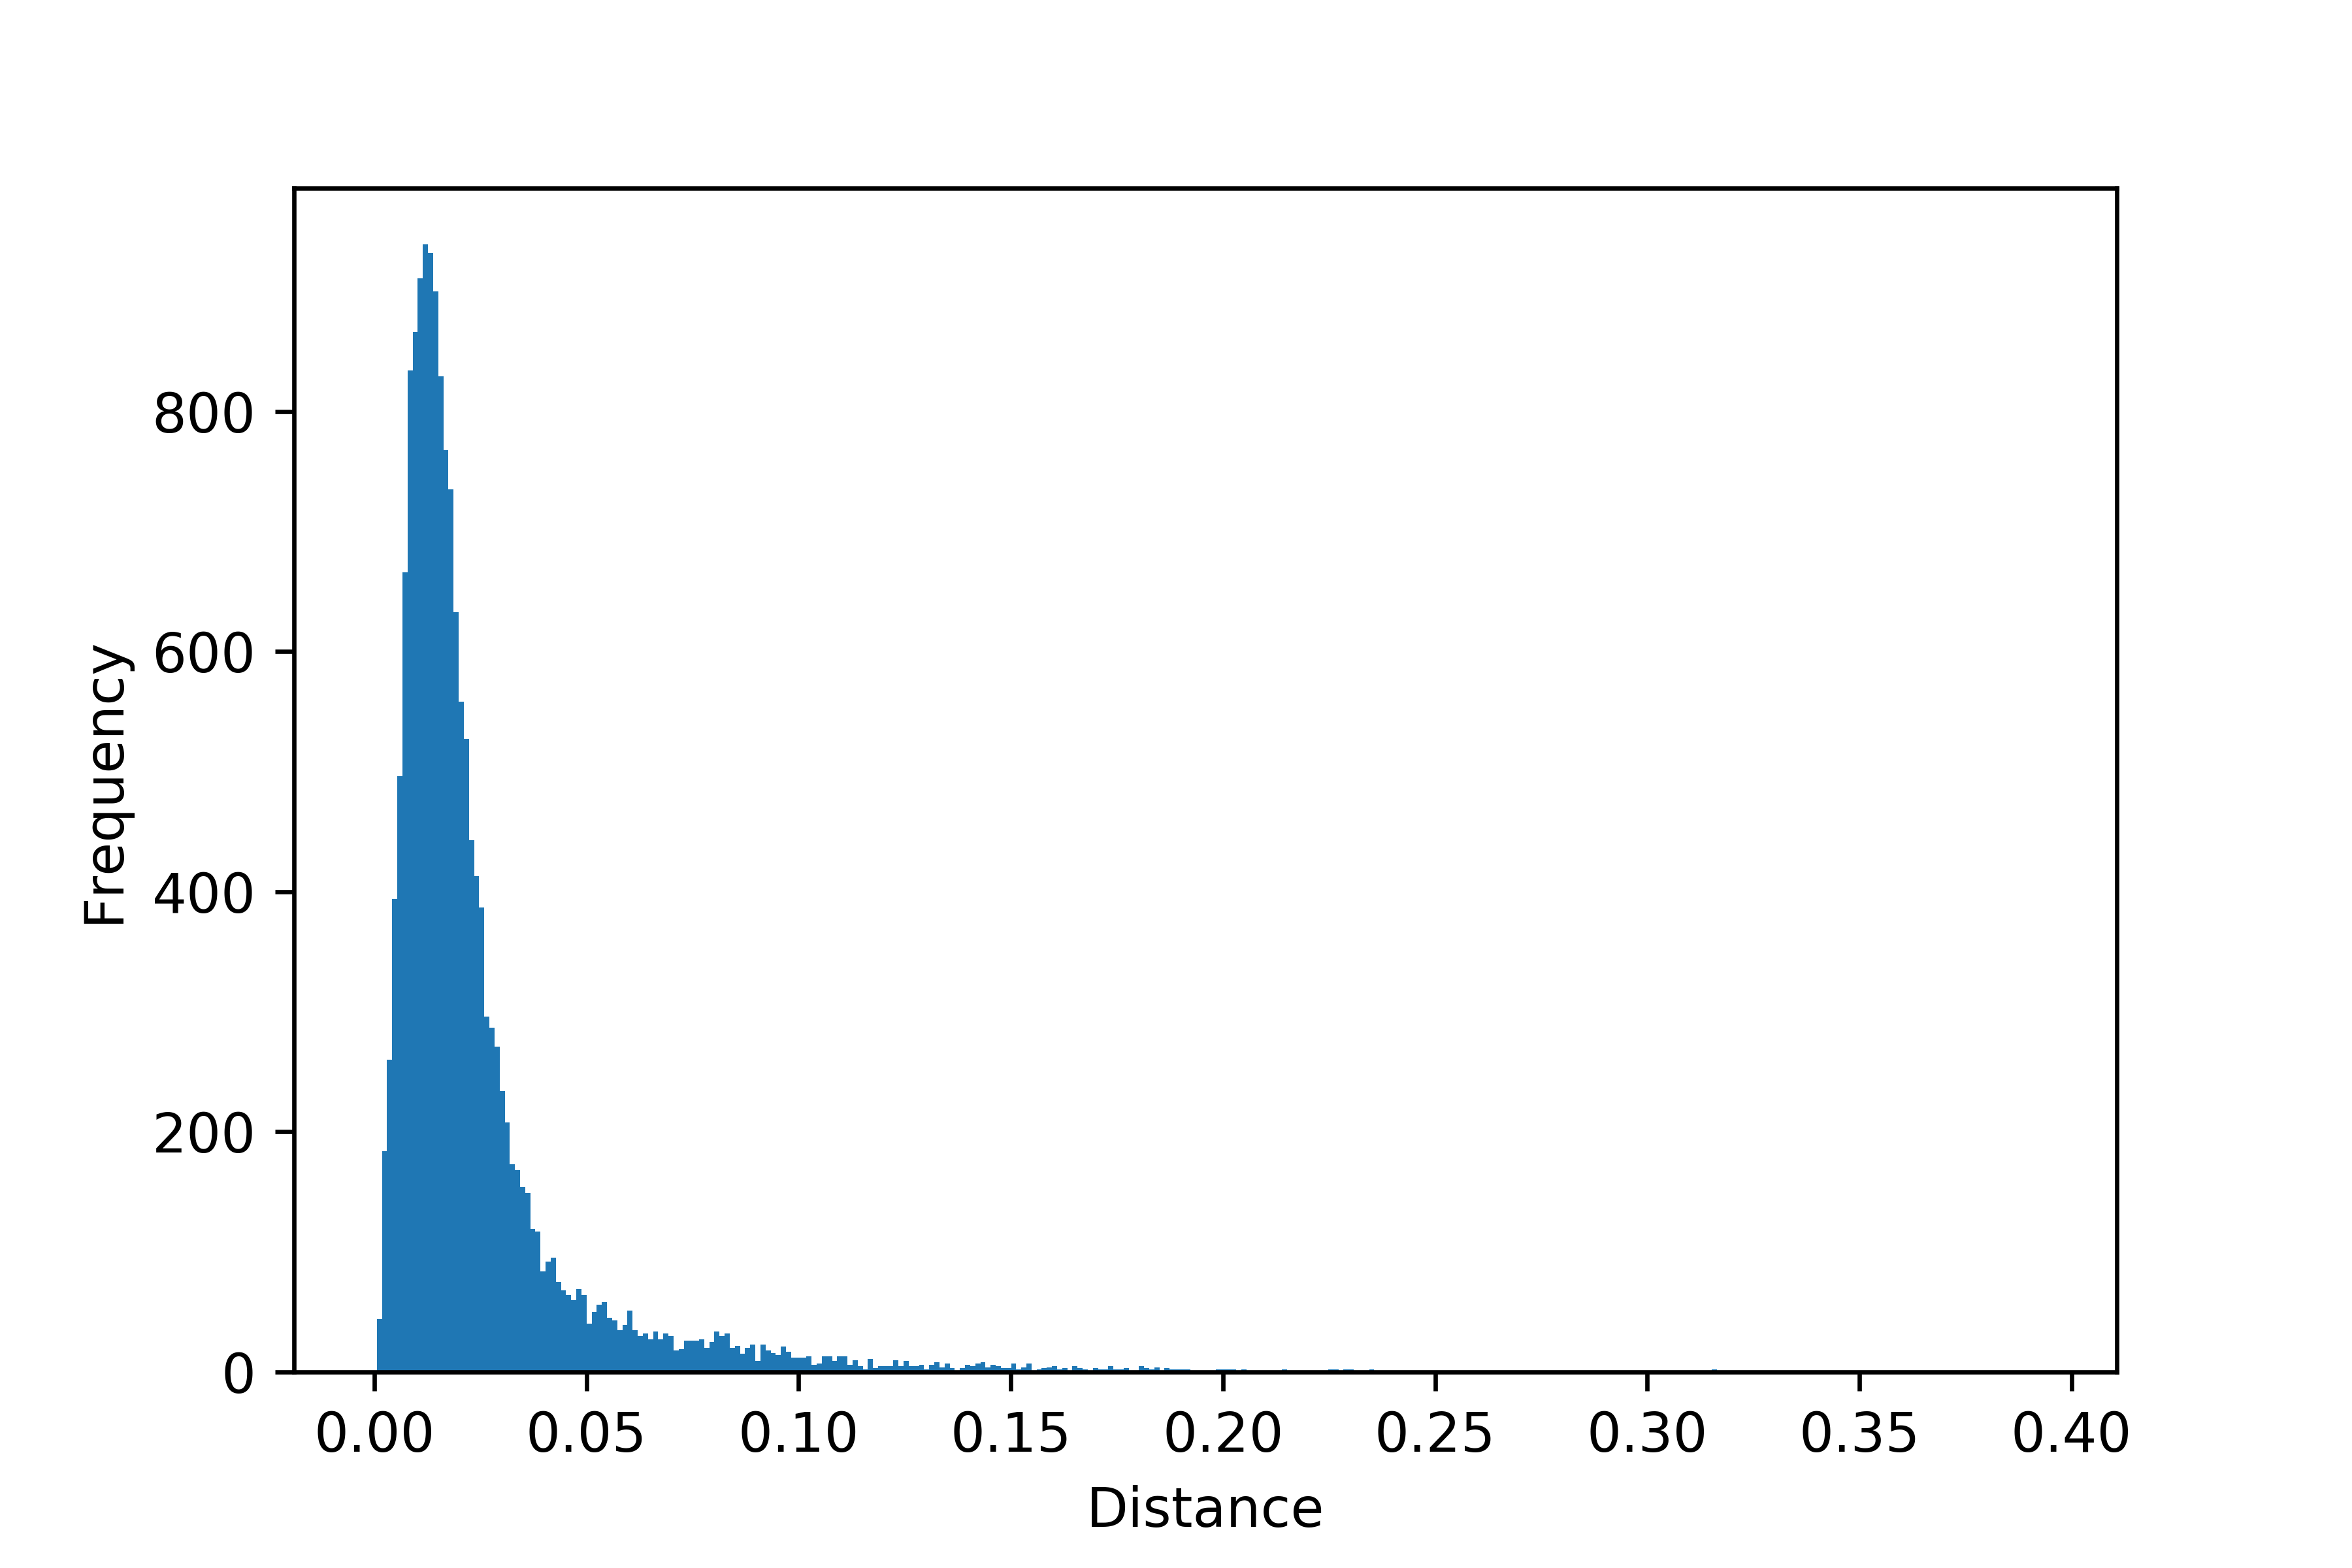
\includegraphics[scale=.90]{118_hist_ICP}
\captionsetup{justification=centering}
\caption{ICP Distances histogram of deformed bundle}
{The histogram shows the frequency of distances between the original pathway points (before local deformation) and correspondent points in the deformed version after applying ICP registration.}
\label{fig:hist_icp_def}
\end{figure}

\begin{figure}[H]
\centering
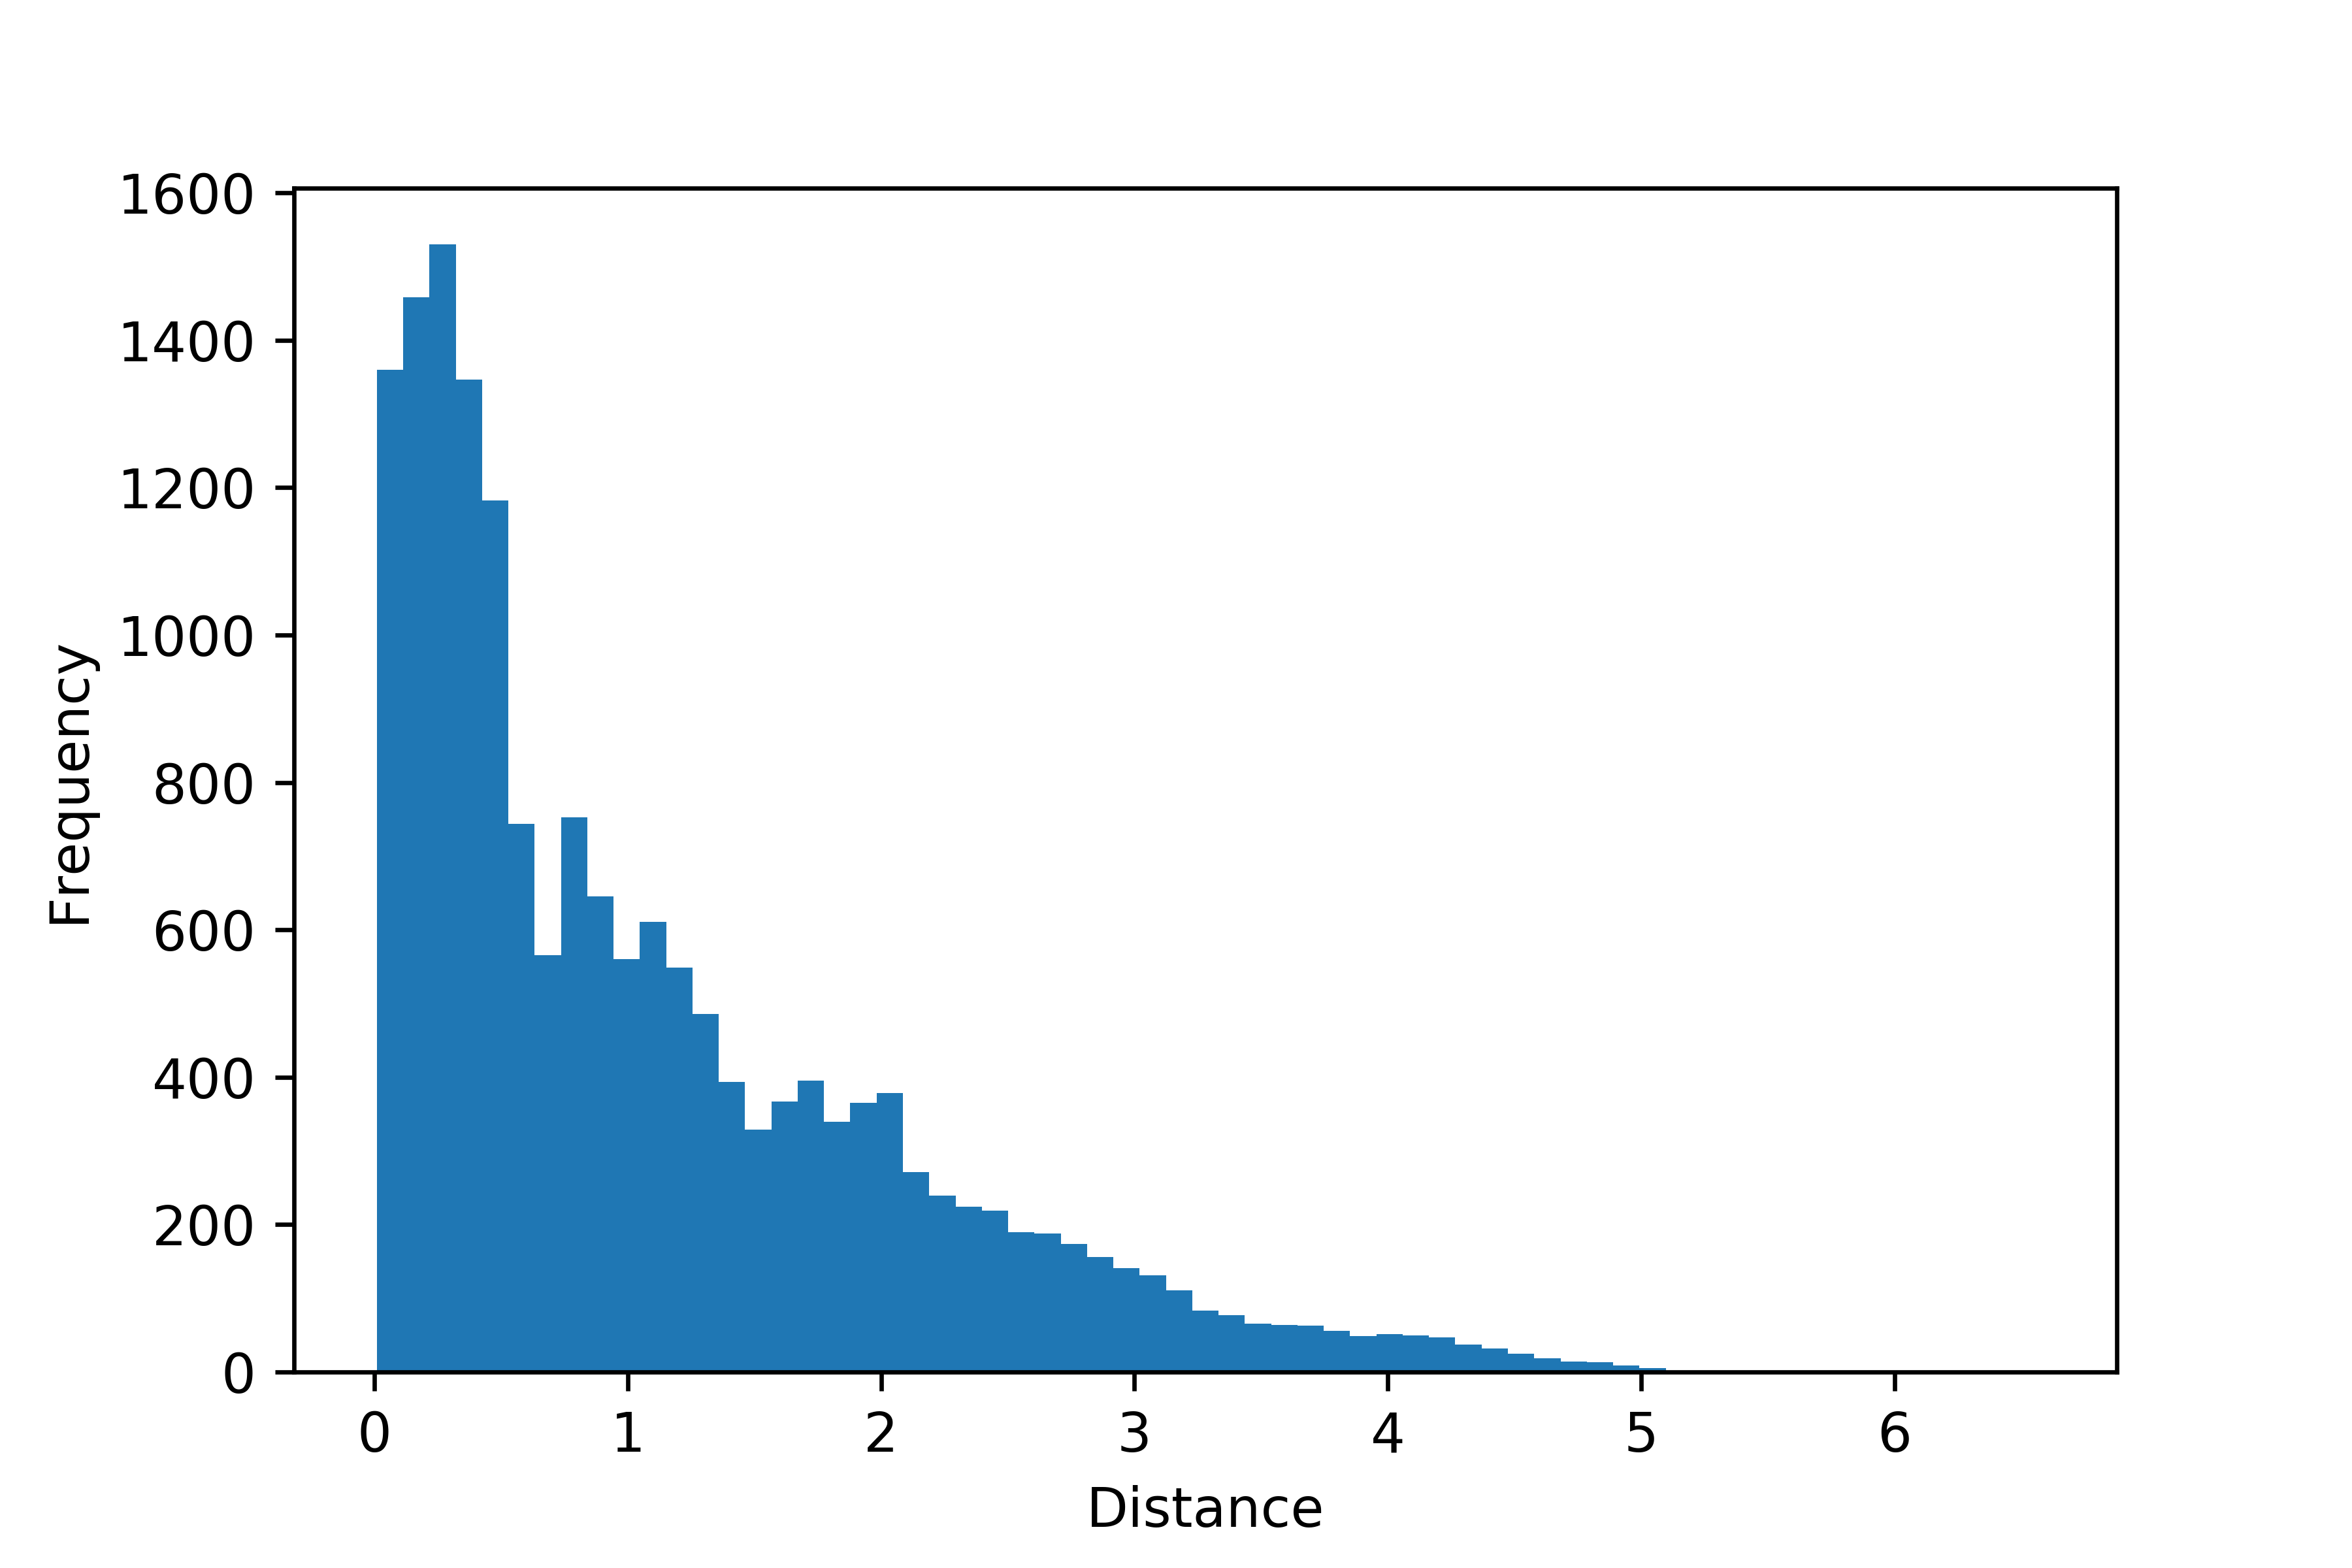
\includegraphics[scale=.90]{118_hist_dipy}
\captionsetup{justification=centering}
\caption{DIPY Distances histogram of deformed bundle}
{The histogram shows the frequency of distances between the original pathway points (before local deformation) and correspondent points in the deformed version after applying DIPY registration.}
\label{fig:hist_dipy_def}
\end{figure}

Finally, we found that our tools can correct the deformation and also locally deform the the shape of the template bundle to find optimal registration, whereas \textit{DIPY} can scale the template bundles to find the optimal size and alignment but can not apply local transformation at least in the current version.

The \textit{DIPY} method is much faster than our method because DIPY is implemented to reduce the number of points used to calculate the distance. In our test, each tract reduced to 20 points rather than the real number of points as shown in table \ref{table:data}. Furthermore, as mentioned in \cite{Garyfallidis2012}, \textit{DIPY} uses a minimum average direct-flip distance (MDF) which considers the tract to tract distance calculation whereas our tool considers the point to point distance calculation. To improve our tool, hierarchical clustering bundles can be done and soft membership alignment can be applied.

\section{Results from different Experiments}
We tested non-rigid ICP registration tool in other pathways and we have sufficient results as shown below.

\begin{figure}[H]
	\centering
	\begin{subfigure}[b]{0.49\textwidth}
	\centering
	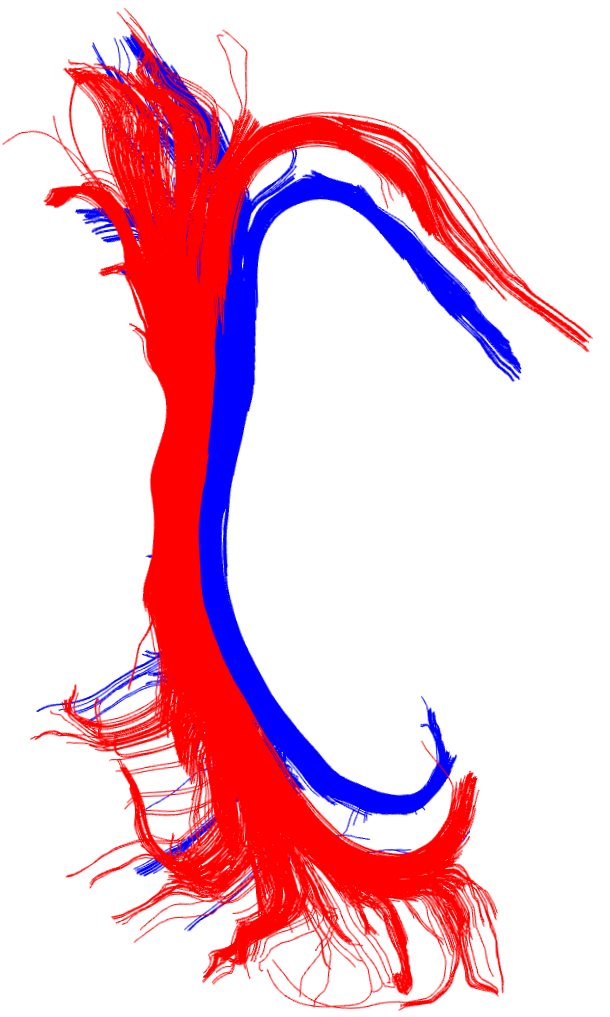
\includegraphics[width=\textwidth]{04_img}
	\caption{Original Orientation}
	\end{subfigure}
	% separate
	\begin{subfigure}[b]{0.49\textwidth}
	\centering
	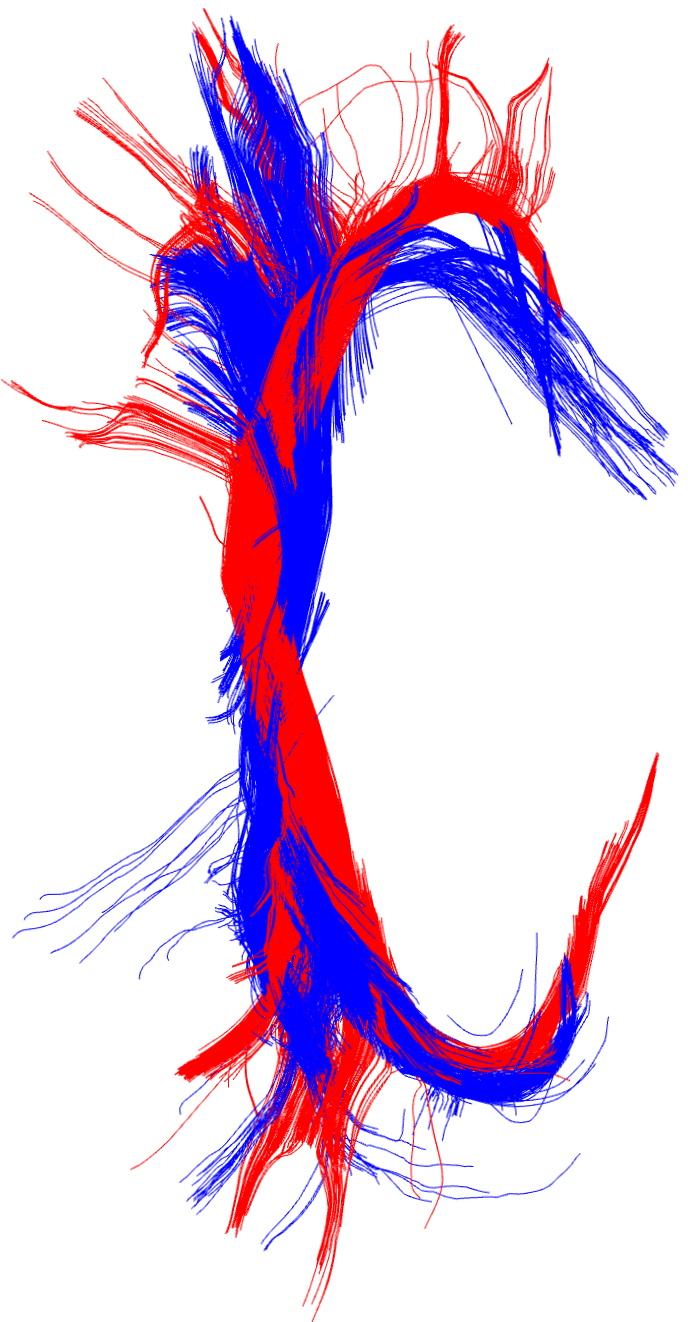
\includegraphics[width=.9\textwidth]{05_img}
	\caption{Orientation after ICP registration}
	\end{subfigure}
\captionsetup{justification=centering}
\caption{Cingulum fiber pathway}
{left (red) and right (blue) side of brain, before and after ICP registration}
\label{fig:pca}
\end{figure}

\begin{figure}[H]
	\centering
	\begin{subfigure}[b]{0.49\textwidth}
	\centering
	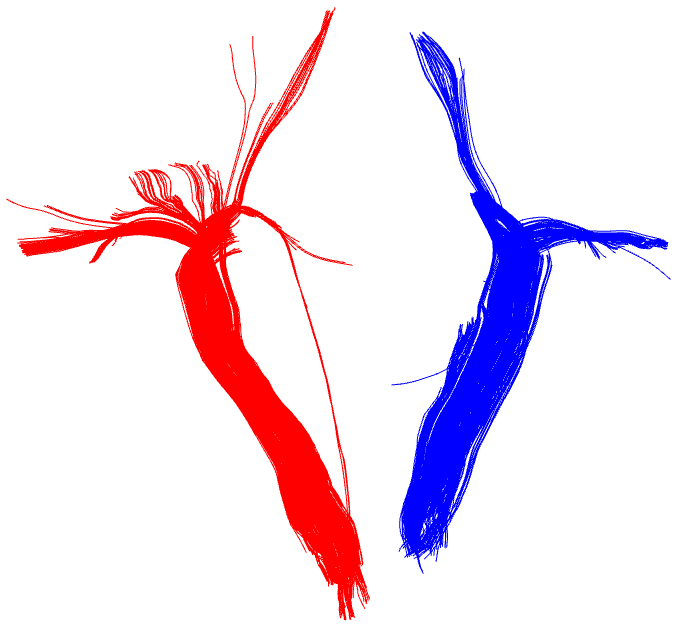
\includegraphics[width=\textwidth]{00_img}
	\caption{Original Orientation}
	\end{subfigure}
	% separate
	\begin{subfigure}[b]{0.49\textwidth}
	\centering
	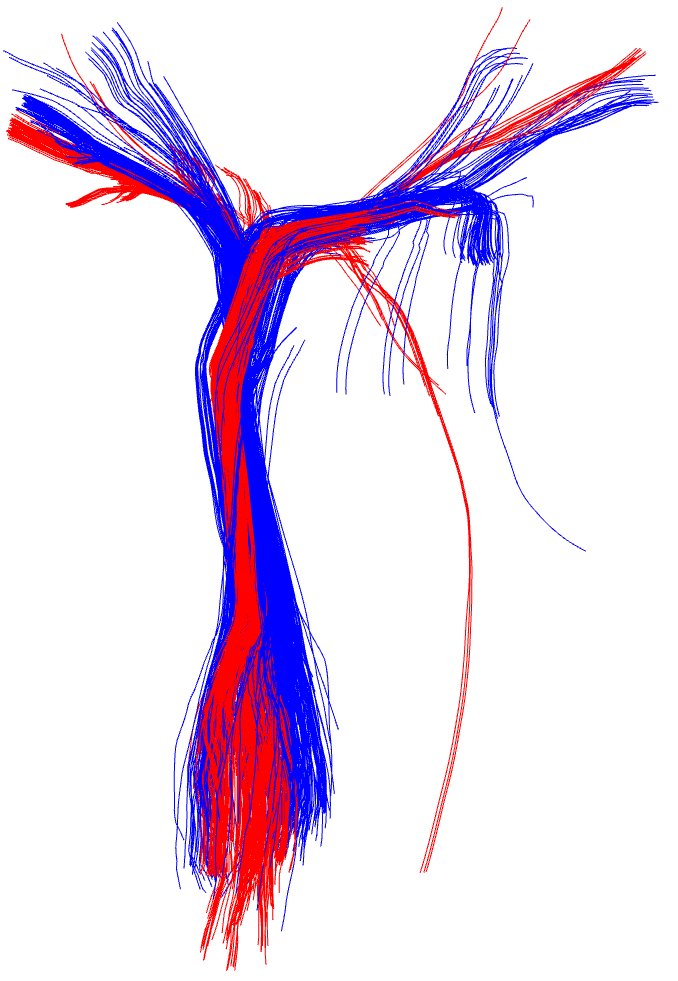
\includegraphics[width=.7\textwidth]{01_img}
	\caption{Orientation after ICP registration}
	\end{subfigure}
\captionsetup{justification=centering}
\caption{Anterior Thalamic Radiation fiber pathway}{ left (red) and right (blue) side of brain, before and after ICP registration}
\label{fig:pca}
\end{figure}

\begin{figure}[H]
	\centering
	\begin{subfigure}[b]{0.49\textwidth}
	\centering
	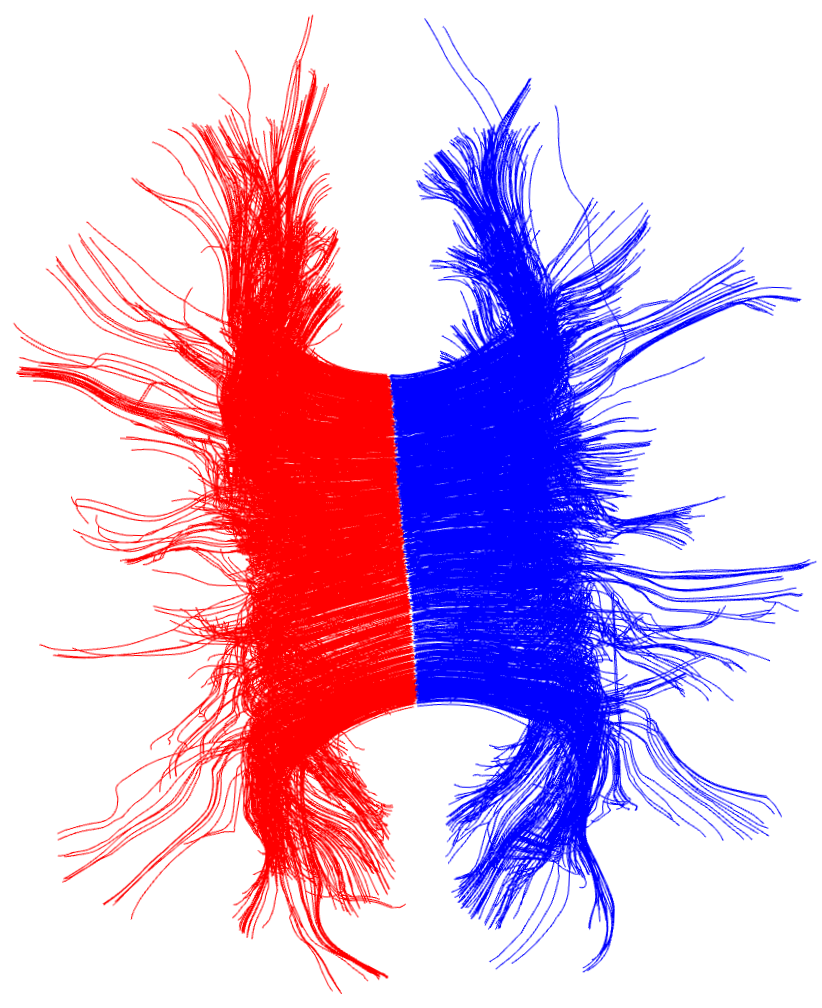
\includegraphics[width=\textwidth]{02_img}
	\caption{Original Orientation}
	\end{subfigure}
	% separate
	\begin{subfigure}[b]{0.49\textwidth}
	\centering
	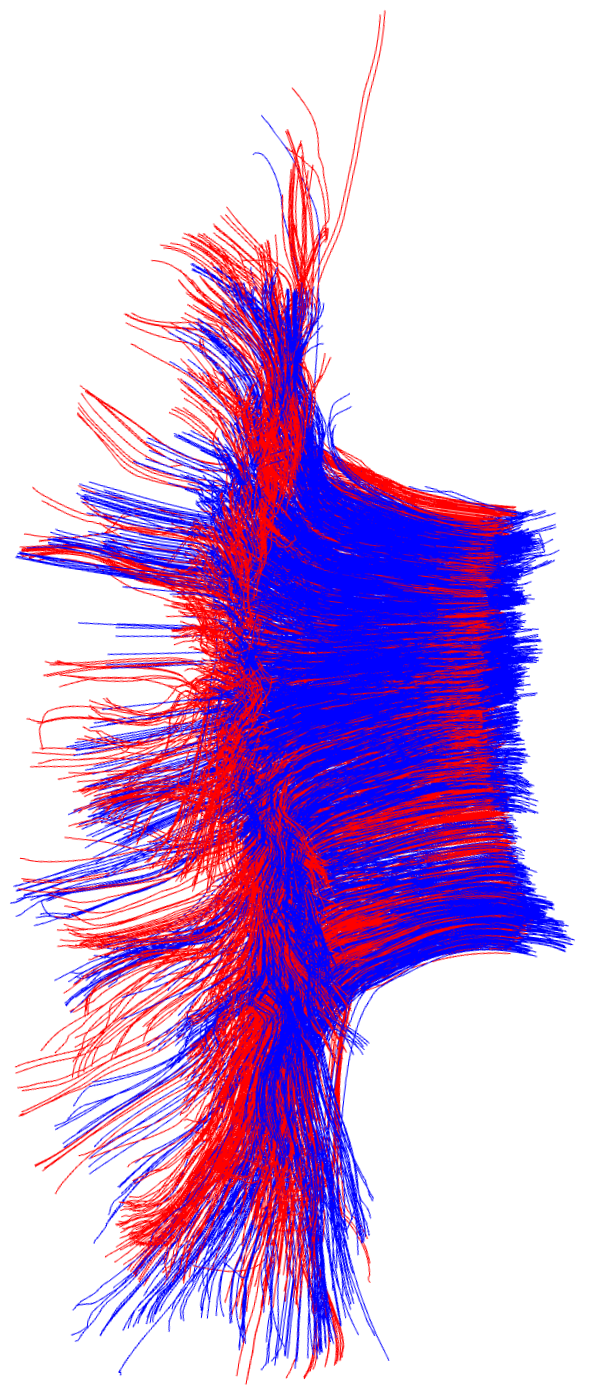
\includegraphics[width=.6\textwidth]{03_img}
	\caption{Orientation after ICP registration}
	\end{subfigure}
\captionsetup{justification=centering}
\caption{The body of Corpus Callosum fiber pathway}{ left (red) and right (blue) side of brain, before and after ICP registration}
\label{fig:pca}
\end{figure}

\begin{figure}[H]
	\centering
	\begin{subfigure}[b]{0.49\textwidth}
	\centering
	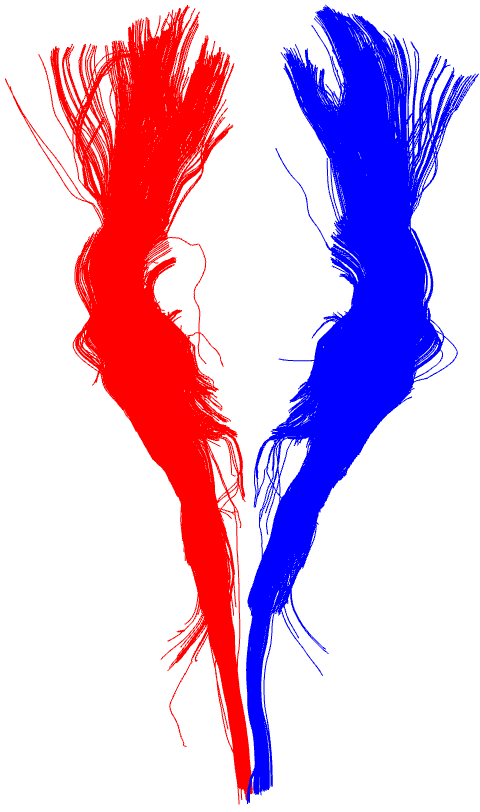
\includegraphics[width=\textwidth]{06_img}
	\caption{Original Orientation}
	\end{subfigure}
	% separate
	\begin{subfigure}[b]{0.49\textwidth}
	\centering
	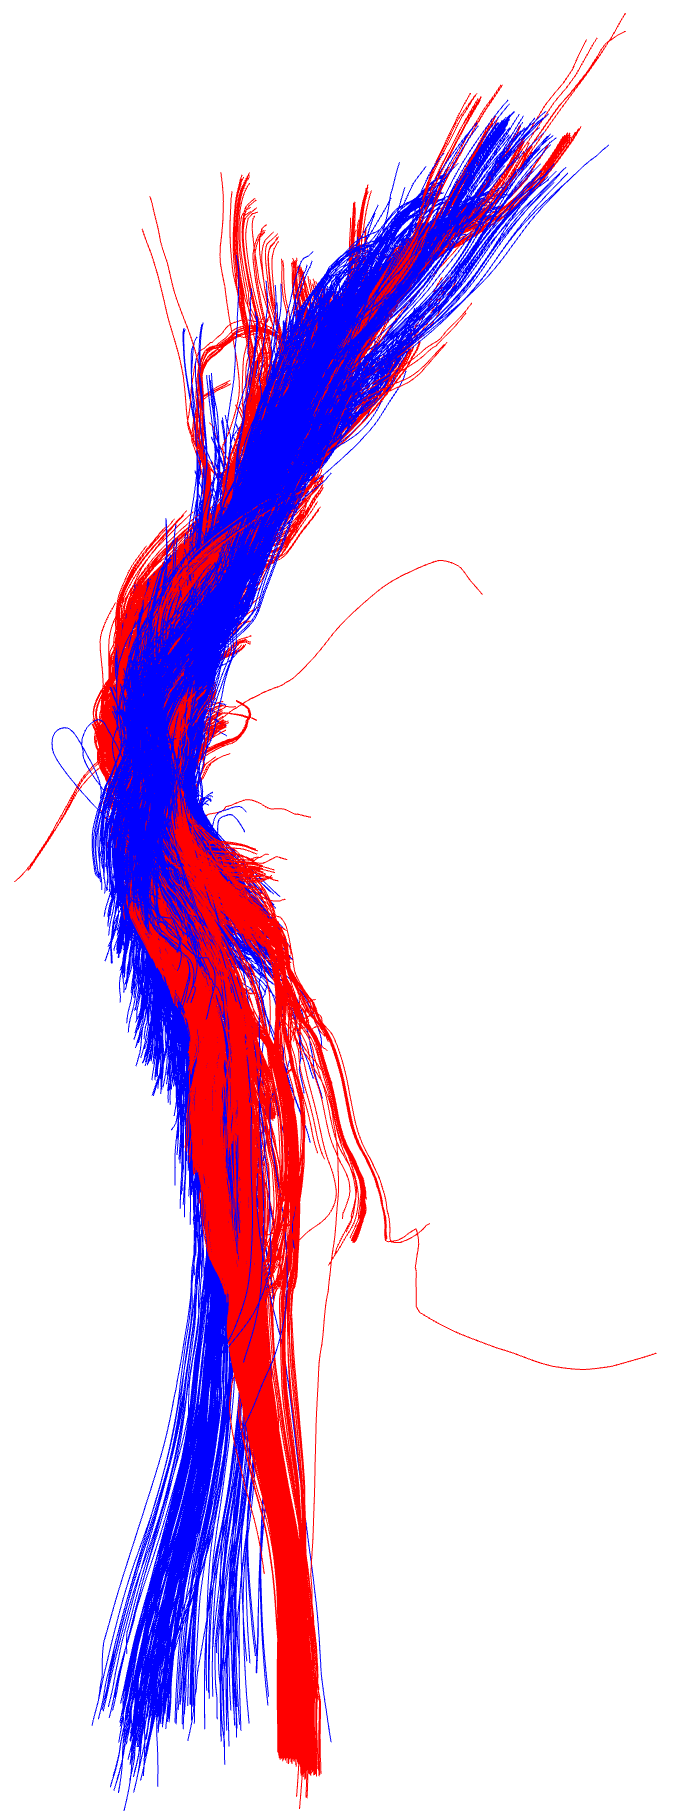
\includegraphics[width=.6\textwidth]{07_img}
	\caption{Orientation after ICP registration}
	\end{subfigure}
\captionsetup{justification=centering}
\caption{Corticospinal Tract fiber pathway}{ left (red) and right (blue) side of brain, before and after ICP registration}
\label{fig:pca}
\end{figure}

\begin{figure}[H]
	\centering
	\begin{subfigure}[b]{0.49\textwidth}
	\centering
	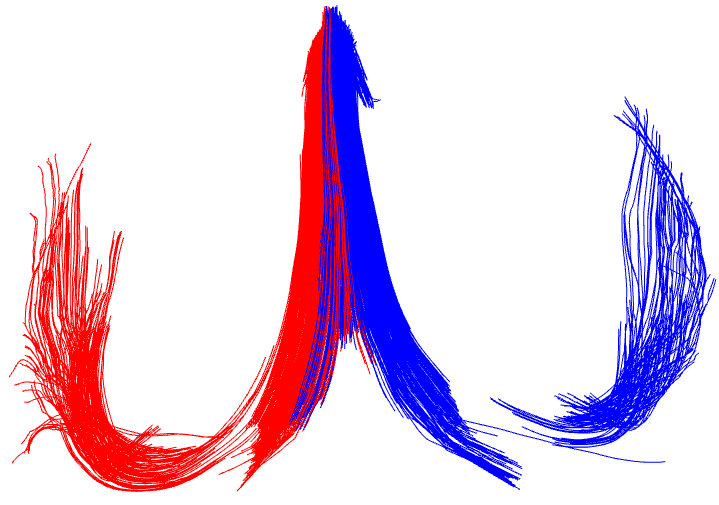
\includegraphics[width=\textwidth]{08_img}
	\caption{Original Orientation}
	\end{subfigure}
	% separate
	\begin{subfigure}[b]{0.49\textwidth}
	\centering
	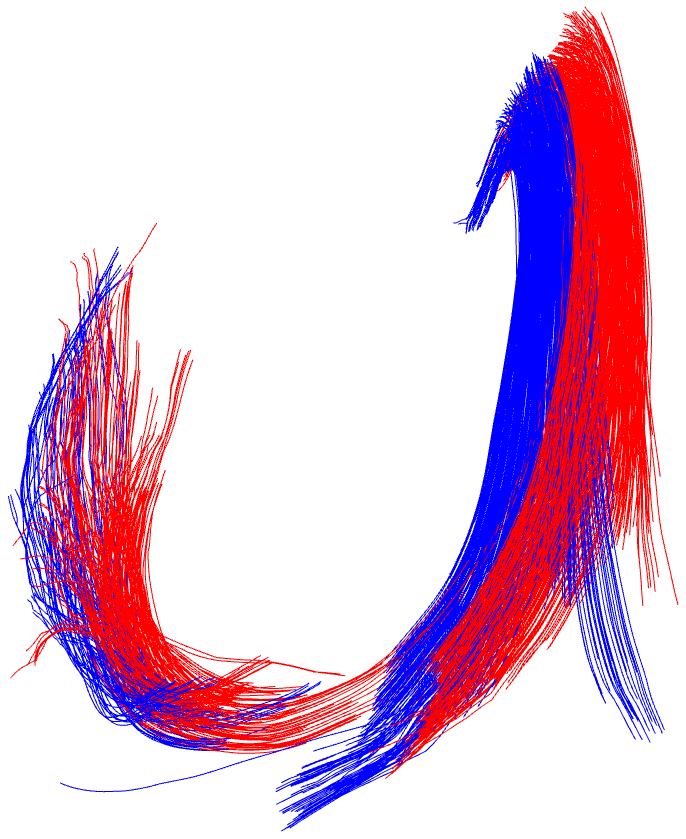
\includegraphics[width=.7\textwidth]{09_img}
	\caption{Orientation after ICP registration}
	\end{subfigure}
\captionsetup{justification=centering}
\caption{Fronix fiber pathway}{ left (red) and right (blue) side of brain, before and after ICP registration}
\label{fig:pca}
\end{figure}

\begin{figure}[H]
	\centering
	\begin{subfigure}[b]{0.49\textwidth}
	\centering
	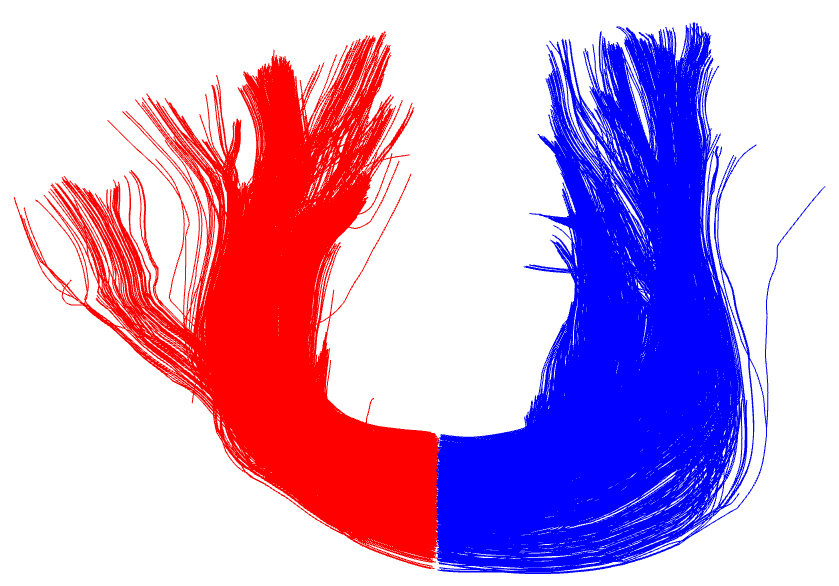
\includegraphics[width=\textwidth]{10_img}
	\caption{Original Orientation}
	\end{subfigure}
	% separate
	\begin{subfigure}[b]{0.49\textwidth}
	\centering
	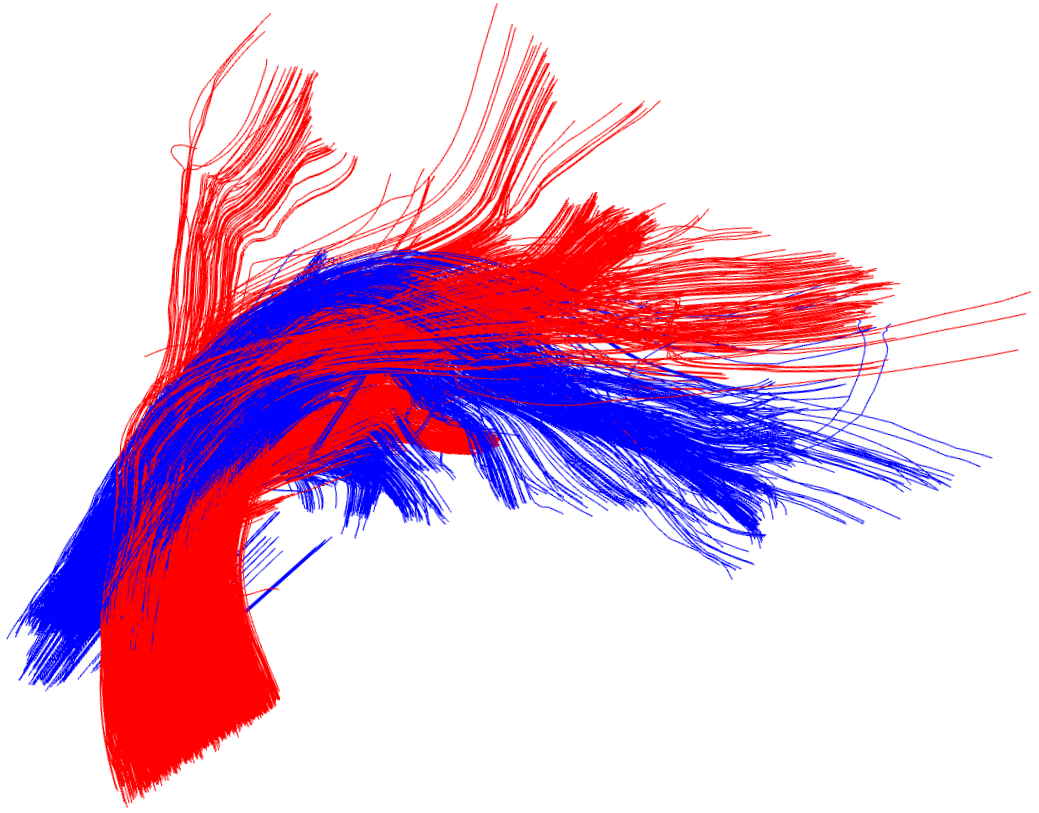
\includegraphics[width=\textwidth]{11_img}
	\caption{Orientation after ICP registration}
	\end{subfigure}
\captionsetup{justification=centering}
\caption{Genu fiber pathway}{ left (red) and right (blue) side of brain, before and after ICP registration}
\label{fig:pca}
\end{figure}

\begin{figure}[H]
	\centering
	\begin{subfigure}[b]{0.49\textwidth}
	\centering
	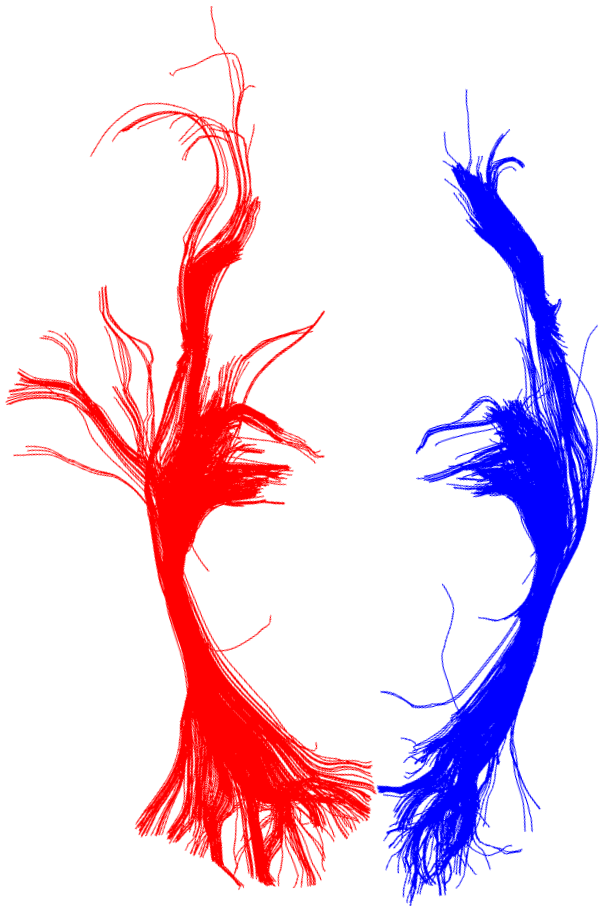
\includegraphics[width=\textwidth]{12_img}
	\caption{Original Orientation}
	\end{subfigure}
	% separate
	\begin{subfigure}[b]{0.49\textwidth}
	\centering
	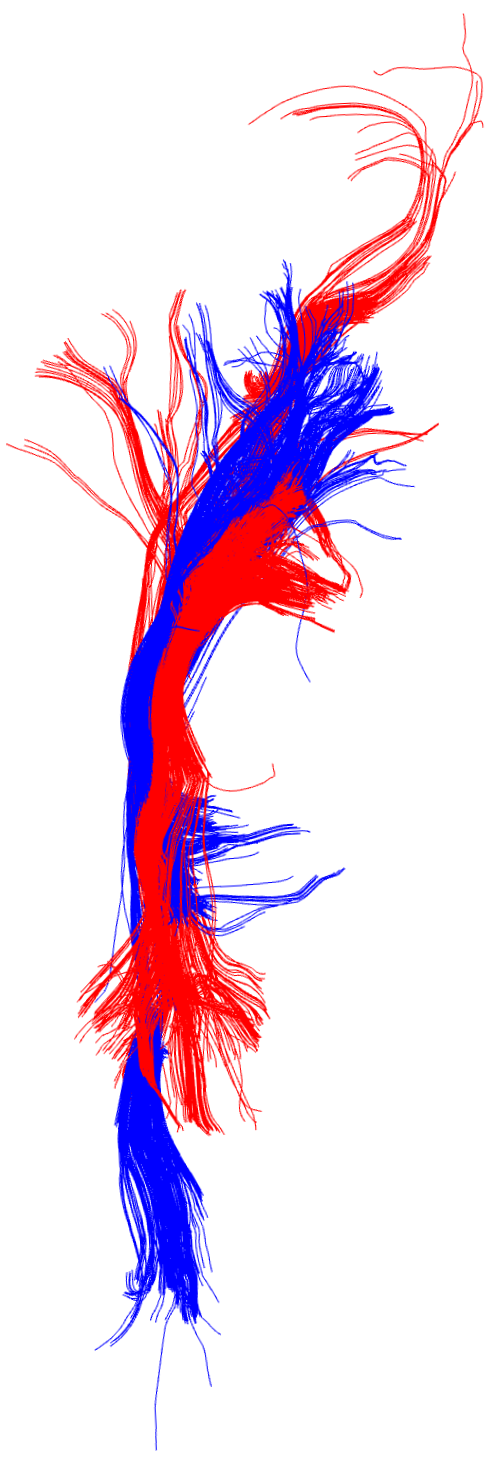
\includegraphics[width=.5\textwidth]{13_img}
	\caption{Orientation after ICP registration}
	\end{subfigure}
\captionsetup{justification=centering}
\caption{Inferior Fronto-occipital Fasciculus fiber pathway}{ left (red) and right (blue) side of brain, before and after ICP registration}
\label{fig:pca}
\end{figure}

\begin{figure}[H]
	\centering
	\begin{subfigure}[b]{0.49\textwidth}
	\centering
	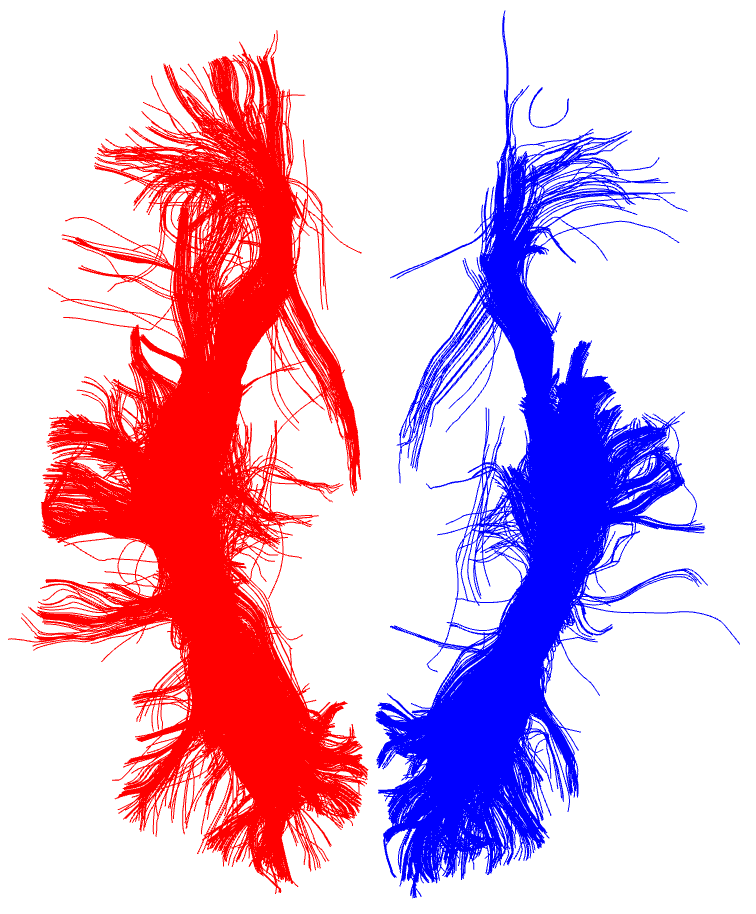
\includegraphics[width=\textwidth]{14_img}
	\caption{Original Orientation}
	\end{subfigure}
	% separate
	\begin{subfigure}[b]{0.49\textwidth}
	\centering
	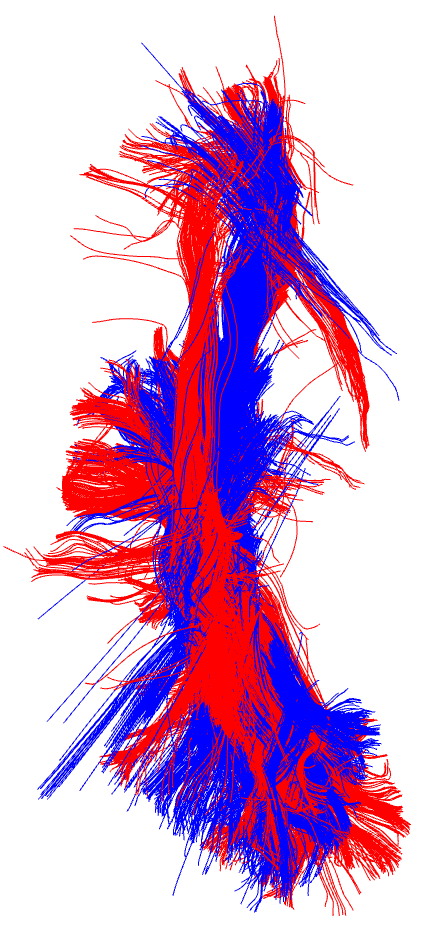
\includegraphics[width=.5\textwidth]{15_img}
	\caption{Orientation after ICP registration}
	\end{subfigure}
\captionsetup{justification=centering}
\caption{Inferior Longtudinal Faciculus fiber pathway}{ left (red) and right (blue) side of brain, before and after ICP registration}
\label{fig:pca}
\end{figure}

% Anterior Thalamic Radiation, The body of Corpus Callosum, Cingulum, Corticospinal Tract, Fronix, Genu, Inferior Fronto-occipital Fasciculus, Inferior Longtudinal Faciculus, Superior Longtudinal Faciculus, Splenium, Ventral Tegmental Area.
\end{document}


